%File principale del documento su cui invocare la compilazione, vedi "istruzioni.txt" per più info

%Preambolo: la parte prima del \begin{document}
\documentclass[12pt,a4paper]{article} %formato del documento e grandezza caratteri

%Input del file metadata.tex della cartella locale "res/"
%lista di comandi presenti in template_latex.tex, da qui posso essere modificati secondo le esigenze

\newcommand{\DocTitle}{Verbale interno 2019-11-18} %variabile usata dal file template_latex.tex per settare il titolo del documento
%\newcommand{\DocAuthor}{Progetto "Predire in Grafana"} %variabile usata dal file template_latex.tex per settare l'autore del documento
\newcommand{\DocDate}{18 Novembre 2019} %variabile usata dal file template_latex.tex; Impostata manualmente, altrimenti ad ogni compilazione viene messa la data del giorno di compilazione.
\newcommand{\DocDesc}{Resoconto dell'incontro del gruppo \textit{VRAM Software} tenutosi in data 2019-11-18} %variabile usata dal file template_latex.tex per settare la descrizione del documento
\newcommand{\ver}{27.0.0} %variabile usata dal file template_latex.tex per settare la versione del documento
\newcommand{\app}{Toffoletto Massimo} %variabile usata dal file template_latex.tex per settare l'approvatore del documento
\newcommand{\red}{Dalla Libera Marco} %variabile usata dal file template_latex.tex per settare il redattore del documento
\newcommand{\test}{Schiavon Rebecca} %variabile usata dal file template_latex.tex per settare il verificatore del documento
\newcommand{\stat}{Approvato} %variabile usata dal file template_latex.tex per settare lo stato del documento
\newcommand{\use}{Interno} %variabile usata dal file template_latex.tex per indicare l'uso del documento %Contiene le varibili che descrivono il documento

%Input di file di configurazione presi dalla cartella "Template-LaTeX/config/", uguali per tutti i documenti
%Attenzione bisogna impostare il percorso del file!
% Tutti i pacchetti usati, da inserire nel preambolo prima delle configurazioni

\usepackage[T1]{fontenc} %Permette la sillabazione su qualsiasi testo contenente caratteri
\usepackage[utf8]{inputenc} %Serve per usare la codifica utf-8
\usepackage[english,italian]{babel} %Imposta italiano lingua principale, inglese secondaria. Es. serve per far apparire "indice" al posto di "contents"

\usepackage{graphicx} %Serve per includere le immagini

\usepackage[hypertexnames=false]{hyperref} %Gestisce i riferimenti/link. Es. Serve per rendere clickabili le sezioni dell'indice

\usepackage{float} %Serve per migliore la definizione di oggetti fluttuanti come figure e tabelle. Es. poter usare l'opzione [H] nelle figure ovvero tenere fissate le immagini che altrimenti LaTeX si sposta a piacere.

\usepackage{listings} %Serve per poter mettere snippets di codice nel testo

\usepackage{lastpage} %Serve per poter introdurre un'etichetta a cui si può fare riferimento Es. piè di pagina; poter fare " \rfoot{\thepage\ di \pageref{LastPage}} "

\usepackage{fancyhdr} %Per header e piè di pagina personalizzati

%Sono alcuni package che potranno esserci utili in futuro
%\usepackage{charter}
%\usepackage{eurosym}
\usepackage{subcaption}
%\usepackage{wrapfig}
%\usepackage{background}
\usepackage{longtable} % tabella che può continuare per più di una pagina
\usepackage[table]{xcolor} % ho dovuto aggiungere table in modo da poter colorare le row della tabella, dava: undefined control sequences
%\usepackage{colortbl}

\usepackage{dirtree} % usato per creare strutte tree-view in stile filesystem
\usepackage{xspace} % usato per inserire caratteri spazio
\usepackage[official]{eurosym}
\usepackage{pdflscape} %Inclusione pacchetti
% Configurazioni varie, da inserire nel preambolo dopo i pacchetti

\hypersetup{hidelinks} %serve per nascondere riquadri rossi che circondano i link 

\lstset{literate= {à}{{\`a}}1 } %Permette di usare lettere accentate nei listings

\pagestyle{fancy} %Imposto stile pagina
\fancyhf{} %Reset, se lo tolgo LaTex mette impostazioni di default (p.es numerazione pagine di default)


\lhead{
\includegraphics[scale=0.25]{img/logo_header.png}} %Left header che compare in ogni pagina
%\rhead{\leftmark} %Nome della top-level structure (p.es. Section in article o Chapter in book) in ogni pagina
\rhead{\DocTitle\ v. \ver} %Right header

\newcommand{\glo}{$_G$} %Comando per aggiungere il pedice G
\newcommand{\glosp}{$_G$ } %Comando per aggiungere il pedice G con spazio

\newcommand\Tstrut{\rule{0pt}{2.6ex}} % top padding
\newcommand\Bstrut{\rule[-0.9ex]{0pt}{0pt}} % bottom padding
\newcommand{\TBstrut}{\Tstrut\Bstrut} % top & bottom padding

%Setto il colore dei link
%\hypersetup{
%	colorlinks,
%	linkcolor=[HTML]{404040},
%	citecolor={purple!50!black},
%	urlcolor={blue!50!black}
%}

%Tabelle e tabulazione (può tornare utile)
%\setlength{\tablcolsep}{10pt}
%\renewcommand{\arraystretch}{1.4}

%Comando per aggiungere le pagine di ogni sezione
%\newcommand{\newSection}[1]{%
%	\input{res/sections/#1}
%}

% Comandi per aggiungere padding a parole contenute nella tabella; è una specie di strut (un carattere invisibile)
%\newcommand\Tstrut{\rule{0pt}{2.6ex}} % top padding
%\newcommand\Bstrut{\rule[-0.9ex]{0pt}{0pt}} % bottom padding
%\newcommand{\TBstrut}{\Tstrut\Bstrut} % top & bottom padding  %Configurazione pacchetti

\begin{document}
	%Input del file "frontmatter" preso dalla cartella "Template-LaTeX/config/", uguale per tutti i documenti
	%Attenzione bisogna impostare il percorso del file!
	% #### FRONTESPIZIO (frontmatter) ####
\setlength{\headheight}{33pt} %Distanzia l'header
\pagenumbering{gobble} %Toglie il numero di pagina
\begin{titlepage}
	\begin{center}
		
\includegraphics[scale=0.6]{img/logo.png} \\ %Logo
		\vspace{0.4cm} %Aggiunge uno spazio verticale di 0.5 cm
		
		{\LARGE Progetto "Predire in Grafana"} \\ %Nome progetto
		\vspace{0.4cm} %Attenzione a mettere il punto e NON la virgola
		
		{\Huge \textbf{\DocTitle}} \\ %Titolo, prende variabile definita in metadata.tex
		\vspace{0.4cm}
		
		\DocDate \\ %Data, prende variabile definita in metadata.tex
		\vspace{0.4cm}
		
		%Allineamento colonne: l=left r=right c=center, 
		%va specificato per ogni colonna
		%Se si vuole la riga tra colonne mettere "|"
		
		\begin{tabular}{r | l} %Elementi colonne separate da "&", le righe finiscono con "\\"
			Versione             & \ver \\
			Approvazione         & \app \\ 
			Redazione            & \red \\
			Verifica             & \test \\
			Stato                & \stat \\
			Uso                  & \use \\
		    Destinato a          & Zucchetti \\
						         & Prof. Vardanega Tullio\\
						         & Prof. Cardin Riccardo\\
			Email di riferimento & vram.software@gmail.com
		\end{tabular}
		\vfill
		\textbf{Descrizione} \\
		\DocDesc
	\end{center}
\end{titlepage}
\clearpage

% #### Impostazione header, footer  e numerazione pagine ####
\pagenumbering{arabic} %Pagine con i numeri arabi + reset a 1
\renewcommand{\footrulewidth}{0.4pt} %Di default footrulewidth==0 e quindi è invisibile, di default \headrulewith==0.4pt
\rfoot{\thepage\ di \pageref{LastPage}} %Pagina n di m, con numeri Arabi; usa il pacchetto "lastpage", in caso non sia possibile usare tale pacchetto mettere al fondo dell'ultima pagina "\label{LastPage}"

% #### Tabella dei log ####
% \textbf = grassetto; \Large = font più grande
% \rowcolors{quanti colori alternare}{colore numero riga pari}{colore numero riga dispari}: colori alternati per riga
% \rowcolor{color}: cambia colore di una riga
% p{larghezza colonna}: p è un tipo di colonna di testo verticalmente allineata sopra, ci sarebbe anche m che è centrata a metà ma non è precisa per questo utilizzo TBStrut; la sintassi >{\centering} indica che il contenuto della colonna dovrà essere centrato
% \TBstrut fa parte di alcuni comandi che ho inserito in config.tex che permetto di aggiungere un po' di padding al testo
% \\ [2mm] : questra scrittura indica che lo spazio dopo una break line deve essere di 2mm
% 

%\setcounter{secnumdepth}{0}
%\hfill \break
%\textbf{\Large{Diario delle modifiche}} \\


\addtocontents{toc}{\protect\setcounter{tocdepth}{0}} %Inserire questo per escludere una sezione dall'indice.

\section*{Registro delle modifiche} %Asterisco per fare sezione non numerata
\rowcolors{2}{gray!25}{gray!15}
\begin{longtable} {
		>{\centering}p{17mm} 
		>{\centering}p{19.5mm}
		>{\centering}p{24mm} 
		>{\centering}p{24mm} 
		>{}p{32mm}}
	\rowcolor{gray!50}
	\textbf{Versione} & \textbf{Data} & \textbf{Nominativo} & \textbf{Ruolo} & \textbf{Descrizione} \TBstrut \\
	14.7.0 & 2020-04-09 & Stantagiuliana Vittorio, Toffoletto Massimo e Spreafico Alessandro & \textit{Progettista}, \textit{Verificatore} e \textit{Responsabile di progetto} & Stesura, verifica e approvazione documento. \TBstrut \\ [2mm]
\end{longtable}

\addtocontents{toc}{\protect\setcounter{tocdepth}{4}} %Inserire questo per ripristinare il normale inserimento delle sezioni nell'indice. 4 significa fino al paragrah
\clearpage

% #### INDICE (tableofcontents) ####
\tableofcontents %Provoca la stampa dell'indice
\clearpage

\setcounter{secnumdepth}{4} %Permette di andare fino alla profondità del paragraph con la numerazione delle sezioni %Imposta il frontespizio, l'indice, header e footer
	
	%\listoftables
	%\pagebreak
	\listoffigures
	\pagebreak
	
	\section{Introduzione}
    \subsection{Scopo del documento}
        L'obiettivo di questo documento è riportare in modo puramente tecnico le scelte architetturali, strutturali e logiche intraprese dal gruppo \textit{VRAM Software} nel corso dello sviluppo del progetto \textit{Predire in Grafana}. Tale allegato sarà quindi corredato di vari diagrammi UML 2.x (classe, package e sequenza) che dimostreranno i vari design pattern adottati, la struttura del prodotto e i suoi scenari di esecuzione.
    \subsection{Scopo del prodotto}
        Il prodotto che il gruppo \textit{VRAM Software} sta approfondendo prevede lo sviluppo di un applicativo esterno e di un plug-in per la piattaforma di analisi Grafana\glosp per la predizione di dati tramite gli algoritmi di support vector machine (SVM) e di regressione lineare (RL). L'applicativo esterno fungerà da trainer generando un file JSON (predittore) partendo da dei dati in CSV a cui viene applicato l'algoritmo di predizione scelto dall'utente. Il file JSON ottenuto sarà poi inserito nel software Grafana tramite l'apposito plug-in e, dopo aver associato i nodi che si vogliono analizzare con i rispettivi predittori, sarà possibile visualizzare la previsione sul grafico della dashboard di Grafana. È inoltre presente la possibilità di salvare suddetti dati su un database InfluxDB. In tal modo il gruppo \textit{VRAM Software} insieme al proponente \textit{Zucchetti} punta ad agevolare l'attività di DevOps fornendo un valido strumento di predizione e monitoraggio dei dati.
    \subsection{Riferimenti}
        \subsubsection{Normativi}
            \begin{itemize}
                \item \textbf{Norme di Progetto}: \textit{Norme di Progetto v. 27.0.0};
                \item \textbf{Capitolato}\glosp \textbf{d'appalto}: \textit{C4 - Zucchetti - Predire in Grafana} \\
                 \url{https://www.math.unipd.it/~tullio/IS-1/2019/Progetto/C4.pdf}.
            \end{itemize}
        \subsection{Informativi}
        \begin{itemize}
        	\item \textbf{Analisi dei Requisiti}: \textit{Analisi dei Requisiti v. 27.0.0}
        \end{itemize}
        \subsection{Tecnici}
            \begin{itemize}
                \item \textbf{TypeScript}: \url{https://www.typescriptlang.org/docs/home.html};
                \item \textbf{JavaScript}: \url{https://developer.mozilla.org/it/docs/Web/JavaScript};
                \item \textbf{AngularJS}: \url{https://docs.angularjs.org/api};
                \item \textbf{React}: \url{https://it.reactjs.org/docs}.
            \end{itemize}
	\pagebreak
	\section{Requisiti di sistema}
Vengono riportati i requisiti minimi per lo sviluppo e l'esecuzione del nostro prodotto. Essi sono uguali sia per l'applicazione esterna che per il plug-in.

\subsection{Requisiti hardware}
I requisiti hardware minimi che devono essere soddisfatti per garantire un corretto funzionamento sono:
\begin{itemize}
	\item RAM: 2 GB;
	\item Memoria interna libera: 5 GB;
	\item Processore: minimo dual core.
\end{itemize}

\subsection{Sistemi operativi}
Il prodotto è stato sviluppato, testato e utilizzato sui seguenti sistemi operativi, perciò è garantita la compatibilità:
\begin{itemize}
	\item Distribuzioni Gnu/Linux post 2019 basate su DEB o RPM;
	\item macOS v. 10.15;
	\item Windows v. 10.
\end{itemize}

\subsection{Browser compatibili}
Il plug-in è stato sviluppato, testato e utilizzato sui seguenti browser perciò ne è garantita la compatibilità:
\begin{itemize}
	\item Google Chrome v. 58;
	\item Mozilla Firefox v. 54;
	\item Microsoft Edge v. 14;
	\item Microsoft Internet Explorer v. 11;
	\item Safari v. 10;
	\item Opera v. 55.
\end{itemize}
Per l'applicazione esterna alla piattaforma Grafana viene utilizzato Chromium che è integrato, dunque non è necessario l'utilizzo di un browser.
Per ottenere un corretto funzionamento del prodotto è richiesta l'abilitazione di Javascript.

	\pagebreak
	\section{Installazione}
Per installare il prodotto\glosp è necessario scaricare il contenuto di questi moduli del repository:
\begin{itemize}
	\item 
\end{itemize}
Terminato lo scaricamento si può procedere all'installazione

\subsection{Applicazione di addestramento esterna}
Per far partire l'applicazione esterna bisogna semplicemente avviare l'eseguibile fornito. Di seguito viene illustrato come.
	\subsubsection{Windows}
	Aprire la cartella "grafana\_configuration\_utility" e fare doppio click sul file "grafana\_configuration\_utility.exe" e si aprirà l'applicazione per l'addestramento.

	\subsubsection{macOS e GNU/Linux}
	\begin{itemize}
		\item aprire la cartella "grafana\_configuration\_utility";
		\item assicurarsi che il file "grafana\_configuration\_utility.sh" sia eseguibile in uno dei modi seguenti:
		\begin{itemize}
			\item fare click con il tasto destro sul file, selezionare proprietà e poi permessi e mettere la spunta su "eseguibile";
			\item aprire un terminale nella cartella "grafana\_configuration\_utility" e dare il seguente comando: 
			\begin{verbatim}
			chmod +x grafana\_configuration\_utility.sh
			\end{verbatim}
		\end{itemize}
		\item aprire un terminale nella cartella BLABLABLA e dare il seguente comando:
		\begin{verbatim}
	    .\grafana_configuration_utility.sh
		\end{verbatim}
	\end{itemize}
\subsection{Grafana}
Per installare Grafana\glo, visitare la pagina \url{https://grafana.com/get}. Qui è possibile trovare il download per macOS, Windows e sistemi operativi GNU/Linux.
\subsubsection{Eseguire il servizio WEB Grafana} Per eseguire il servizio WEB Grafana\glo, aprire la cartella "bin" dell'installazione Grafana\glosp ed a seconda del sistema operativo eseguire:
\begin{itemize}
	\item \textbf{Windows}: doppio click sul file "grafana-server";
	\item \textbf{Linux e Mac}: eseguire in una shell il comando:
	\begin{verbatim}
	./grafana-server web
	\end{verbatim}
\end{itemize}
Collegarsi quindi con un browser all'indirizzo \url{http://localhost:3000/}. Le credenziali richieste al primo avvio sono username "admin" e password "admin".
\begin{center}
	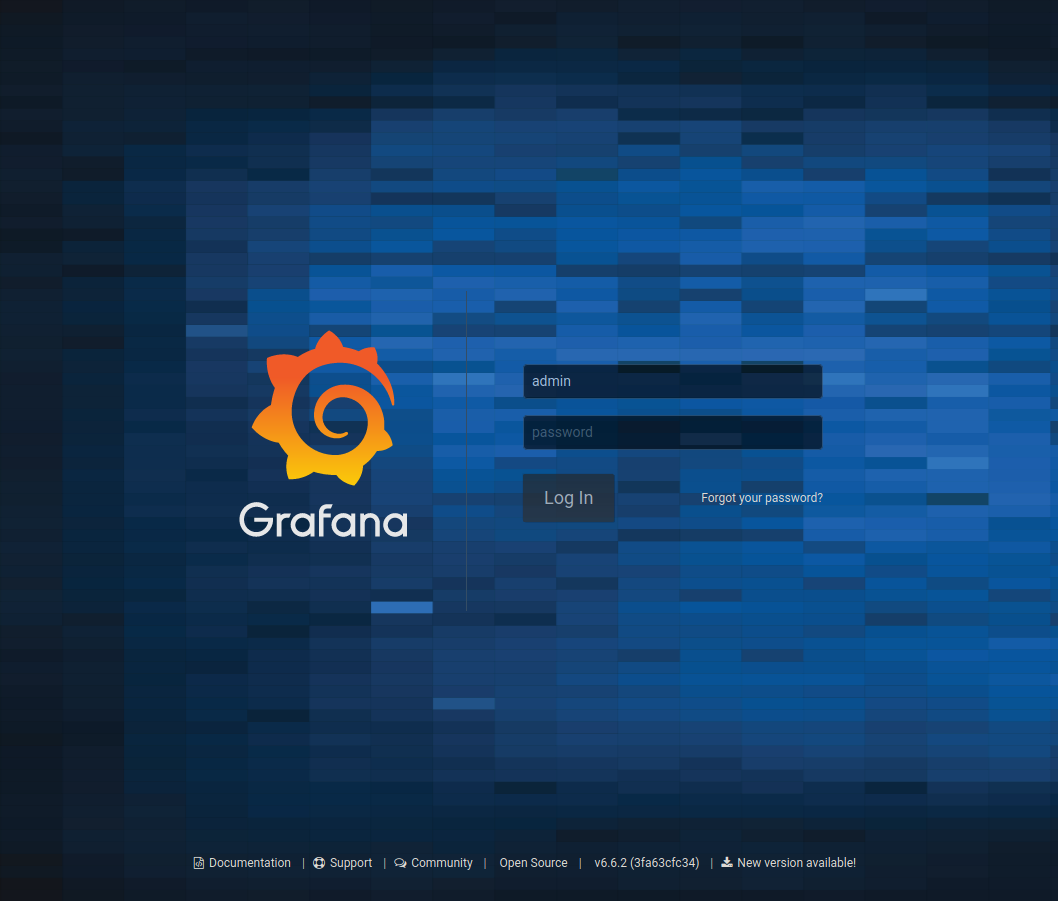
\includegraphics[width=10cm,height=\textheight,keepaspectratio]{img/grafana-login.png}
\end{center}

\subsection{Plug-in di Grafana}
Per poter utilizzare il plug-in bisogna copiare la cartella "grafana\_prediction\_plugin" (scaricata dal link a inizio sezione) all'interno della cartella "data/plugins" dell'installazione Grafana\glo. \\
Bisogna poi trovare il plug-in "Grafana prediction plugin"
\begin{center}
	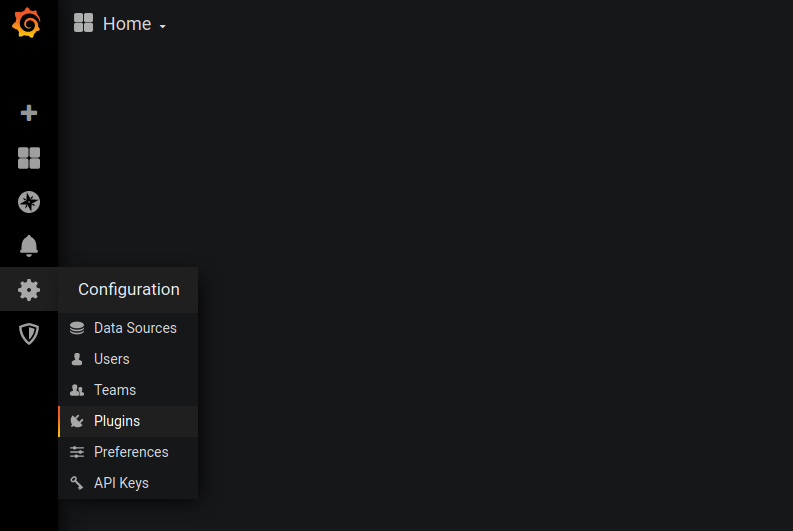
\includegraphics[width=10cm]{img/inserimento-plugin1.png}
\end{center}

\begin{center}
	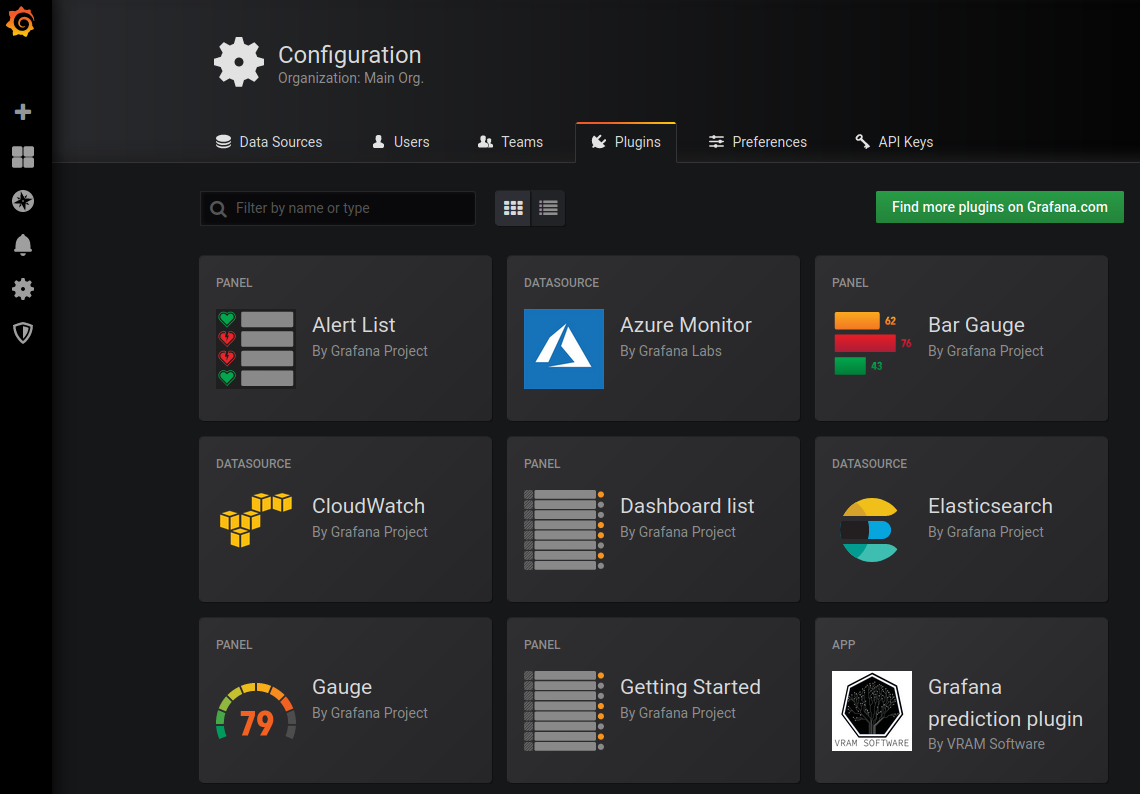
\includegraphics[width=10cm]{img/inserimento-plugin2.png}
\end{center}

Infine è necessario abilitare il plug-in: una volta cliccato su "Grafana prediction plugin", sarà sufficiente aprire la tab "Config" e cliccare sul pulsante "Enable".

\begin{center}
	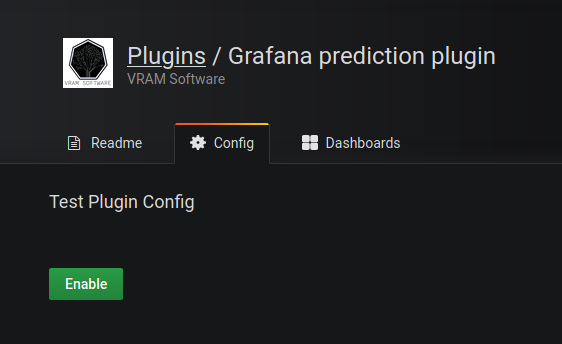
\includegraphics[width=10cm]{img/inserimento-plugin3.png}
\end{center}


	\pagebreak
	\section{Utilizzo plug-in}
    \subsection{Abilitazione plug-in}
        Dopo aver installato il plug-in nella piattaforma Grafana\glo, la prima cosa da fare è abilitarlo. È quindi necessario connettersi alla pagina principale di Grafana\glosp e successivamente bisogna:
        \begin{enumerate}
            \item dal menù laterale cliccare sulla voce "Plugins" dentro alla sezione "Configuration" (icona con l'ingranaggio);
            \item selezionare e cliccare l'app "Grafana prediction plugin";
            \item infine, nella pagina seguente (pagina di configurazione del plug-in), cliccare il pulsante "Enable".
        \end{enumerate}
        \begin{figure}[H]
            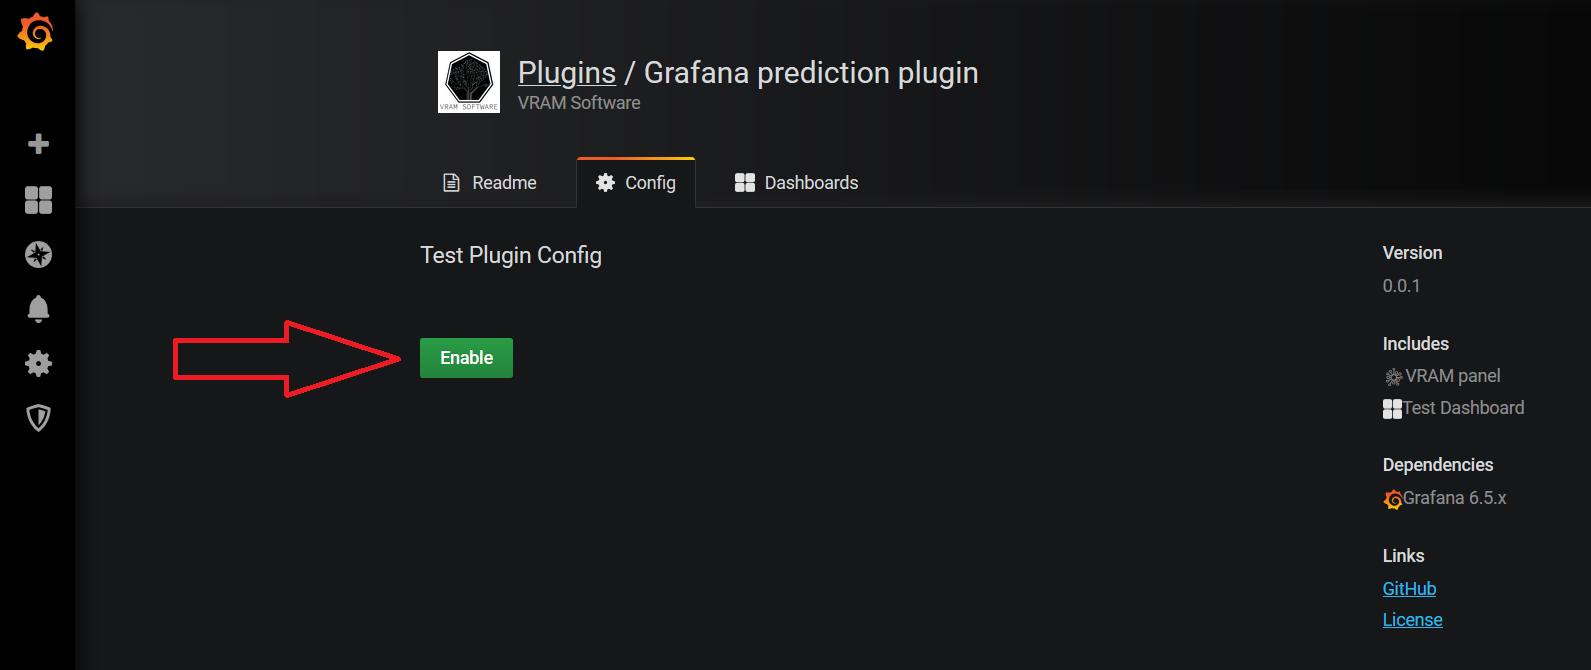
\includegraphics[width=\textwidth,height=\textheight,keepaspectratio]{img/abilitazione_plug-in.png}
            \caption{Pagina di configurazione del plug-in atta all'abilitazione}
        \end{figure}
    \subsection{Aggiunta panel}
        Ad abilitazione avvenuta, la prima cosa da fare per interagire con il plug-in è aggiungere il pannello di \textit{VRAM Software} in una dashboard\glo. Per farlo bisogna seguire i seguenti passi:
        \begin{enumerate}
            \item dal menù laterale cliccare la voce "Dashboard" dentro alla sezione "Create" (simbolo "+");
            \item scegliere l'opzione "Choose Visualization" dal riquadro;
            \item infine selezionare il pannello "VRAM panel".
        \end{enumerate}
        \begin{figure}[H]
            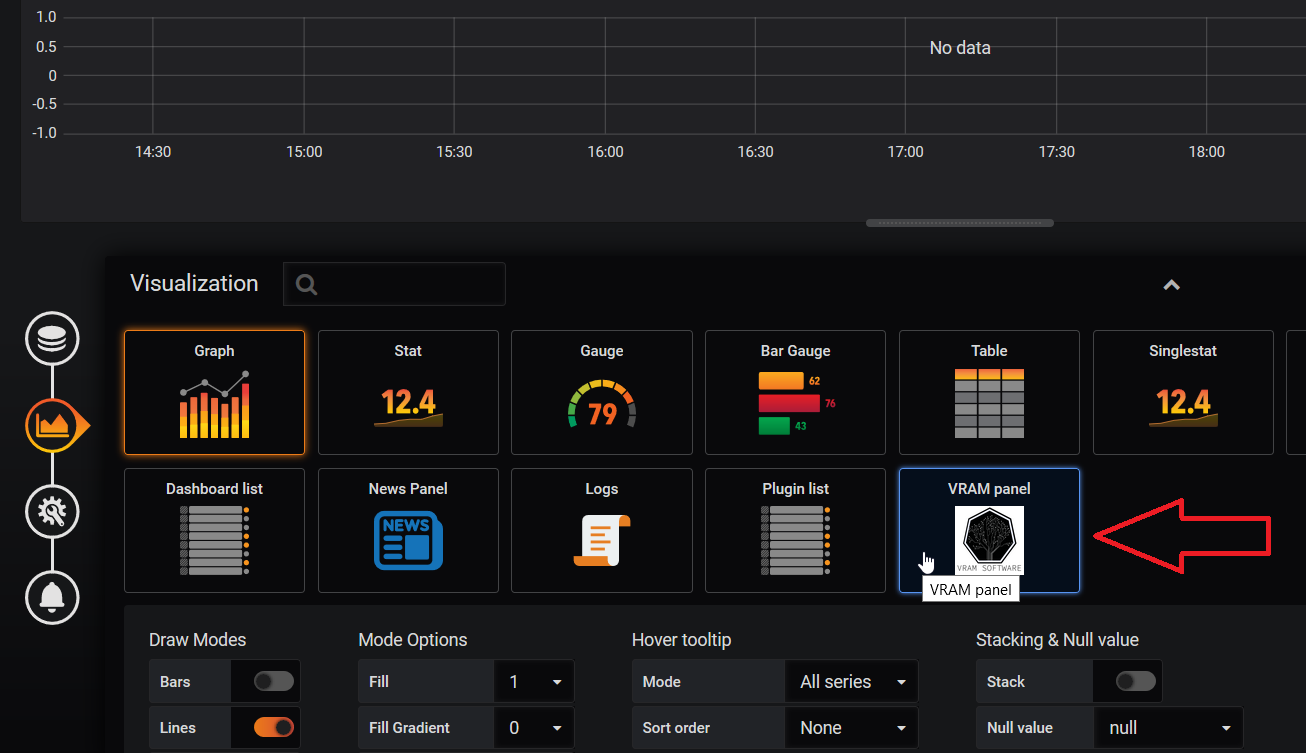
\includegraphics[width=\textwidth,height=\textheight,keepaspectratio]{img/aggiunta_plug-in.png}
            \caption{Pagina della scelta visualizzazione della dashboard}
        \end{figure}
    \subsection{Modificare il pannello}
        Una volta aggiunto il pannello, sarà possibile modificare la sua configurazione. Per fare ciò si devono seguire i seguenti passaggi dalla homepage di Grafana\glo:
        \begin{enumerate}
            \item dal menù laterale cliccare sulla voce "Manage" dentro alla sezione "Dashboard" (icona con i quattro riquadri);
            \item cliccare il nome della dashboard\glosp a cui si vuole accedere (eventualmente usare i vari filtri offerti da Grafana\glosp per facilitare la ricerca);
            \item infine ci si troverà di fronte al grafico desiderato dove bastera premere sul nome e selezionare la voce "Edit".
        \end{enumerate}
        \begin{figure}[H]
            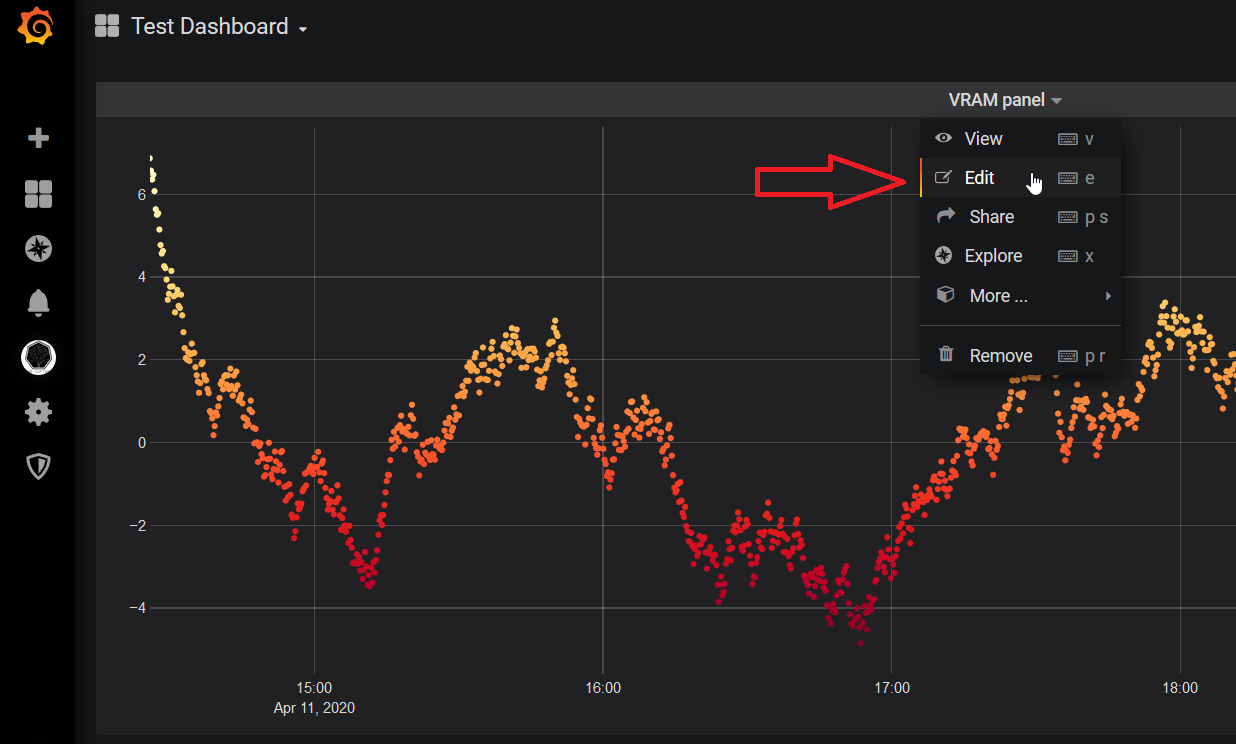
\includegraphics[width=\textwidth,height=\textheight,keepaspectratio]{img/modificare_pannello.png}
            \caption{Selezione opzioni pannello}
        \end{figure}
        In alternativa, se la dashboard\glosp è stata usata recentemente, è possibile trovare il suo nome direttamente in homepage. Diventa quindi sufficiente seguire le istruzioni sopracitate dal punto numero 2.
    \subsection{Importazione e rimozione file JSON dei predittori}
        Nel pannello è possibile aggiungere un file JSON contenente la configurazione degli algoritmi di predizione precedentemente calcolata tramite l'applicativo esterno. Per farlo bisogna seguire i seguenti passi:
        \begin{enumerate}
            \item entrare nella sezione di modifica del pannello;
            \item nel menù laterale cliccare la voce "Visualization" (icona del grafico);
            \item nel riquadro "Import json file" cliccare il pulsante "Upload .json file";
            \item selezionare il file desiderato dal file chooser e premere "Apri".
        \end{enumerate}
        \begin{figure}[H]
            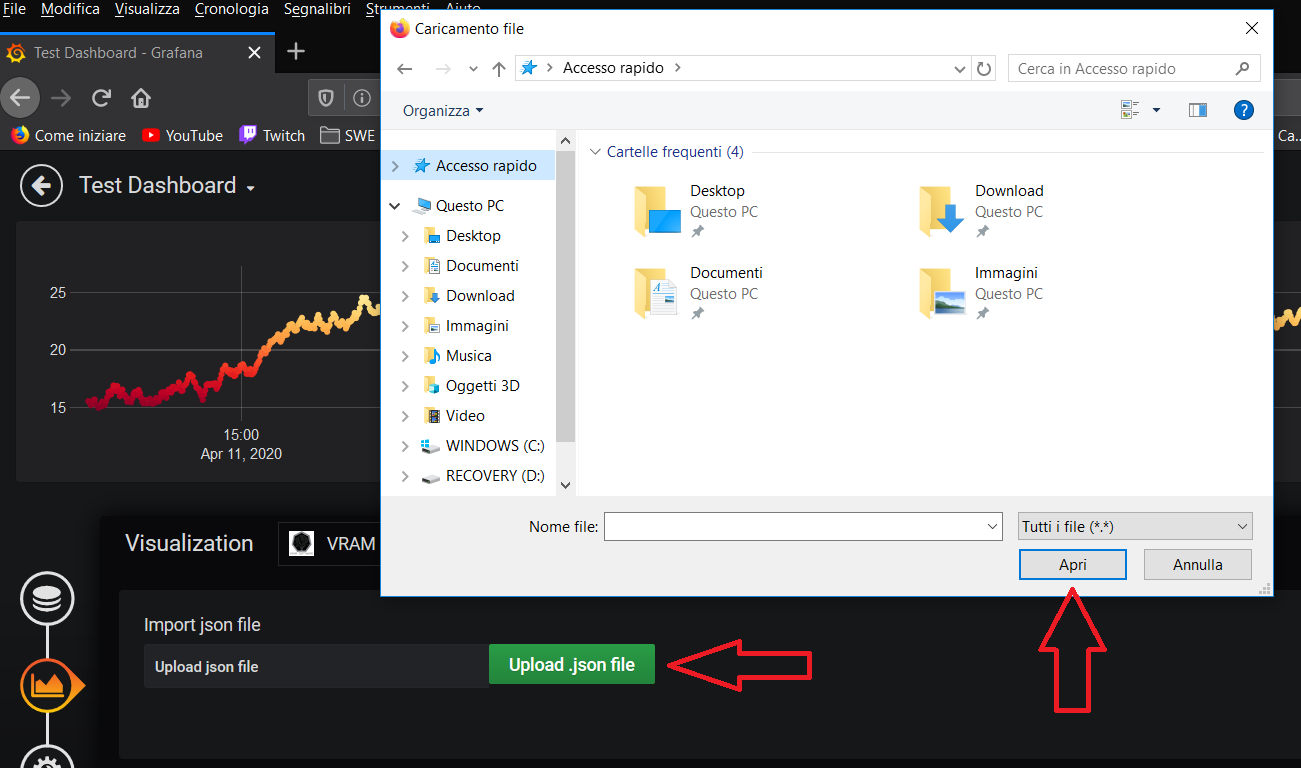
\includegraphics[width=\textwidth,height=\textheight,keepaspectratio]{img/importazione_e_rimozione_JSON.png}
            \caption{Riquadro "Import json file"}
        \end{figure}
        Caricato il file JSON sarà poi possibile rimuoverlo premendo sul pulsante "Remove" situato sempre nel riquadro "Import json file".
    \subsection{Associazione dei nodi al flusso dati}
        Se è stato caricato un file JSON valido, è possibile associare il flusso dati su Grafana\glosp ai predittori\glosp inseriti. Le istruzioni da seguire sono le seguenti:
        \begin{enumerate}
            \item entrare nella sezione di modifica del pannello;
            \item nel menù laterale cliccare la voce "Visualization" (icona del grafico);
            \item nel riquadro "Select query associations" saranno presenti delle label che indicano i predittori e dei selettori che permetteranno di scegliere il flusso dati desiderato;
            \item una volta scelta l'associazione per attuarla basterà premere il pulsante "Confirm".
        \end{enumerate}
        \begin{figure}[H]
            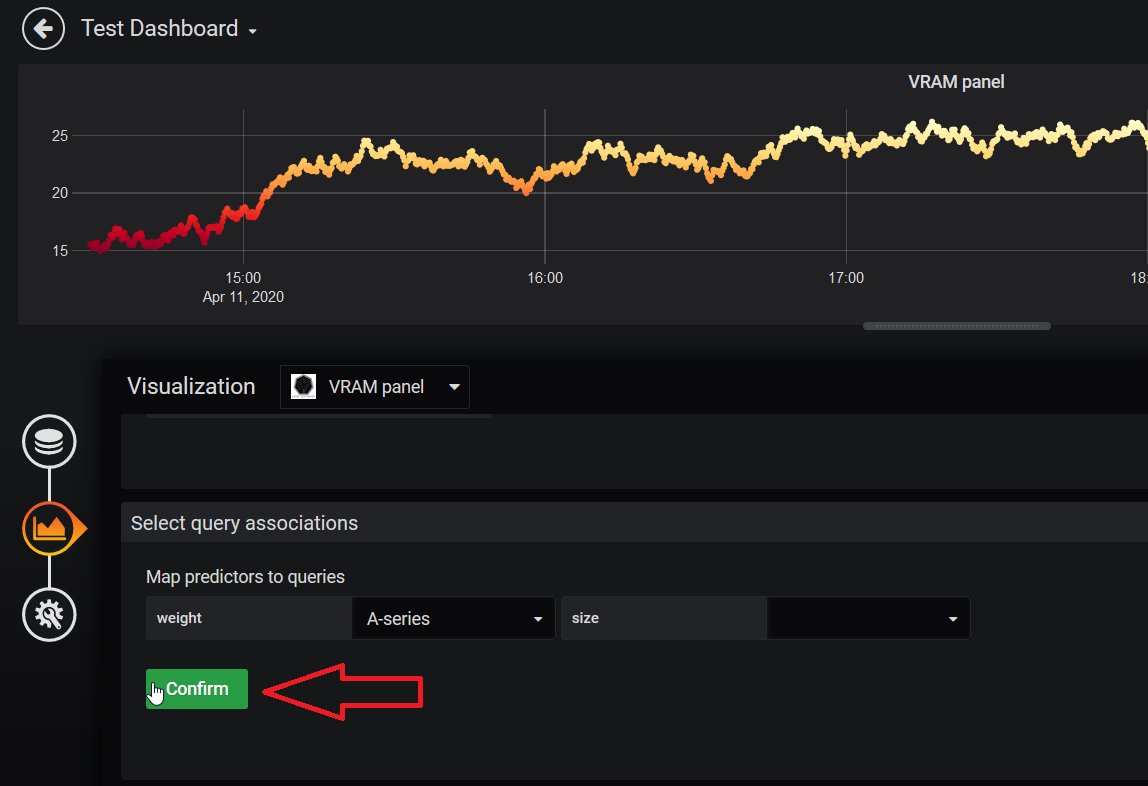
\includegraphics[width=\textwidth,height=\textheight,keepaspectratio]{img/associazione_nodi.png}
            \caption{Riquadro "Select query associations"}
        \end{figure}
    \subsection{Scrittura sul database InfluxDB}
        Se è stata configurata correttamente una datasource\glosp relativa ad un database InfluxDB\glo, è possibile salvare i risultati della previsione. Per configurare la connessione col database InfluxDB\glosp bisogna:
        \begin{enumerate}
            \item entrare nella sezione di modifica del pannello;
            \item nel menù laterale cliccare la voce "Visualization" (icona del grafico);
            \item nel riquadro "Configure influxDB destination" bisogna inserire:
            \begin{enumerate}
                \item datasource\glosp di tipo InfluxDB\glo;
                \item nome del database;
                \item measurement;
                \item field key.
            \end{enumerate}
            \item una volta inseriti i dati basterà premere il tasto "Confirm" per convalidare il collegamento.
        \end{enumerate}
        \begin{figure}[H]
            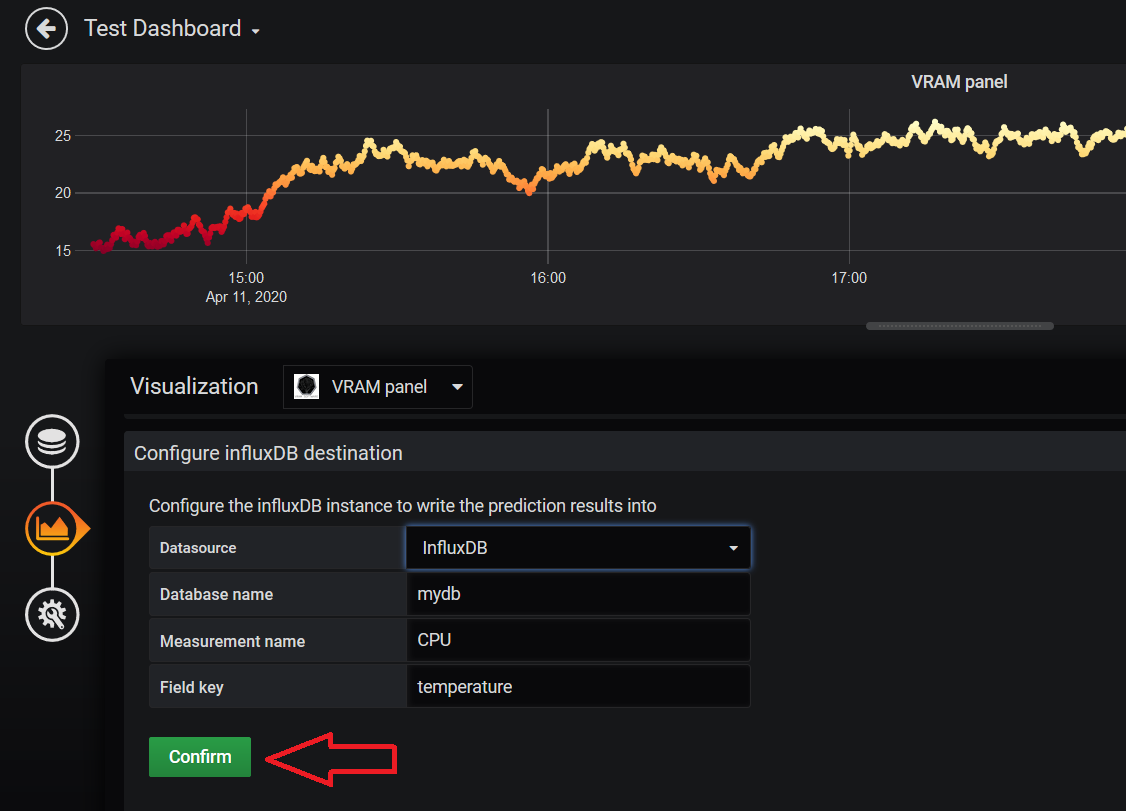
\includegraphics[width=\textwidth,height=\textheight,keepaspectratio]{img/scrittura_InfluxDB.png}
            \caption{Riquadro "Configure influxDB destination"}
        \end{figure}
    \subsection{Modifiche di visualizzazione del grafico}
        Per quanto riguarda il grafico sono presenti due riquadri, "Display" e "Traces", che offrono molte opzioni per personalizzare l'aspetto del grafico. Inoltre, come impostazioni predefinita, è presente una toolbar direttamente sul grafico per compiere azioni veloci come l'aggiornamento automatico della scala degli assi o l'esportazione dell'area visualizzata. Infine è possibile aggiungere nuove tracce per visualizzare molteplici query su uno stesso grafico.
        \begin{figure}[H]
            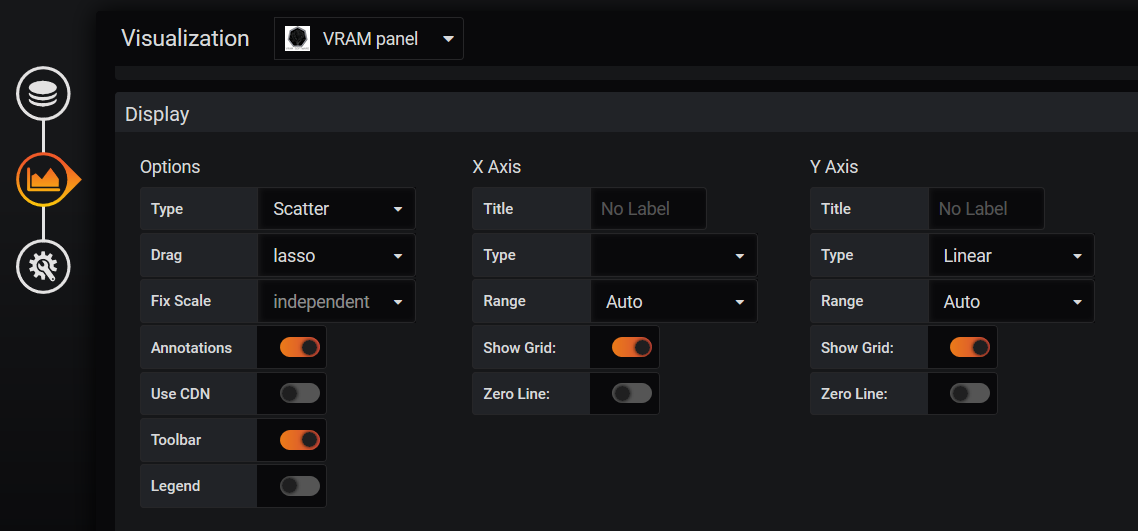
\includegraphics[width=\textwidth,height=\textheight,keepaspectratio]{img/display.png}
            \caption{Riquadro "Display"}
        \end{figure}
        \begin{figure}[H]
            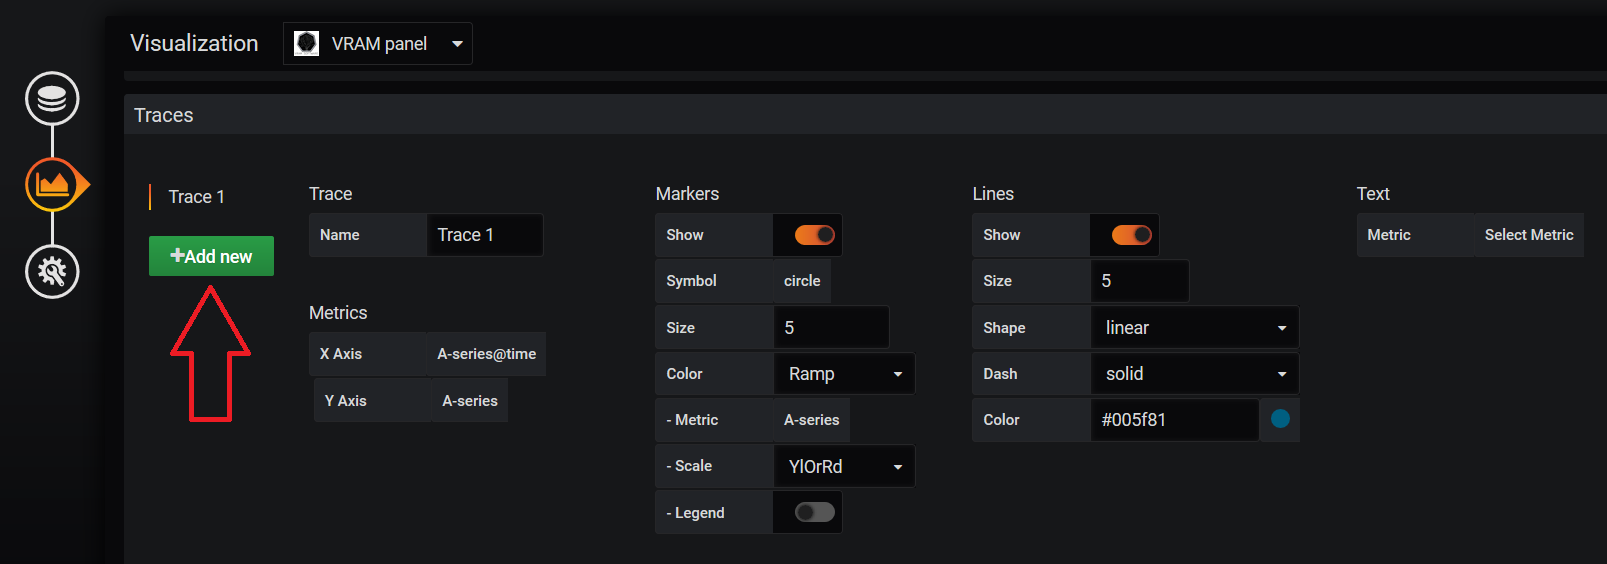
\includegraphics[width=\textwidth,height=\textheight,keepaspectratio]{img/traces.png}
            \caption{Riquadro "Traces"}
        \end{figure}
        \begin{figure}[H]
            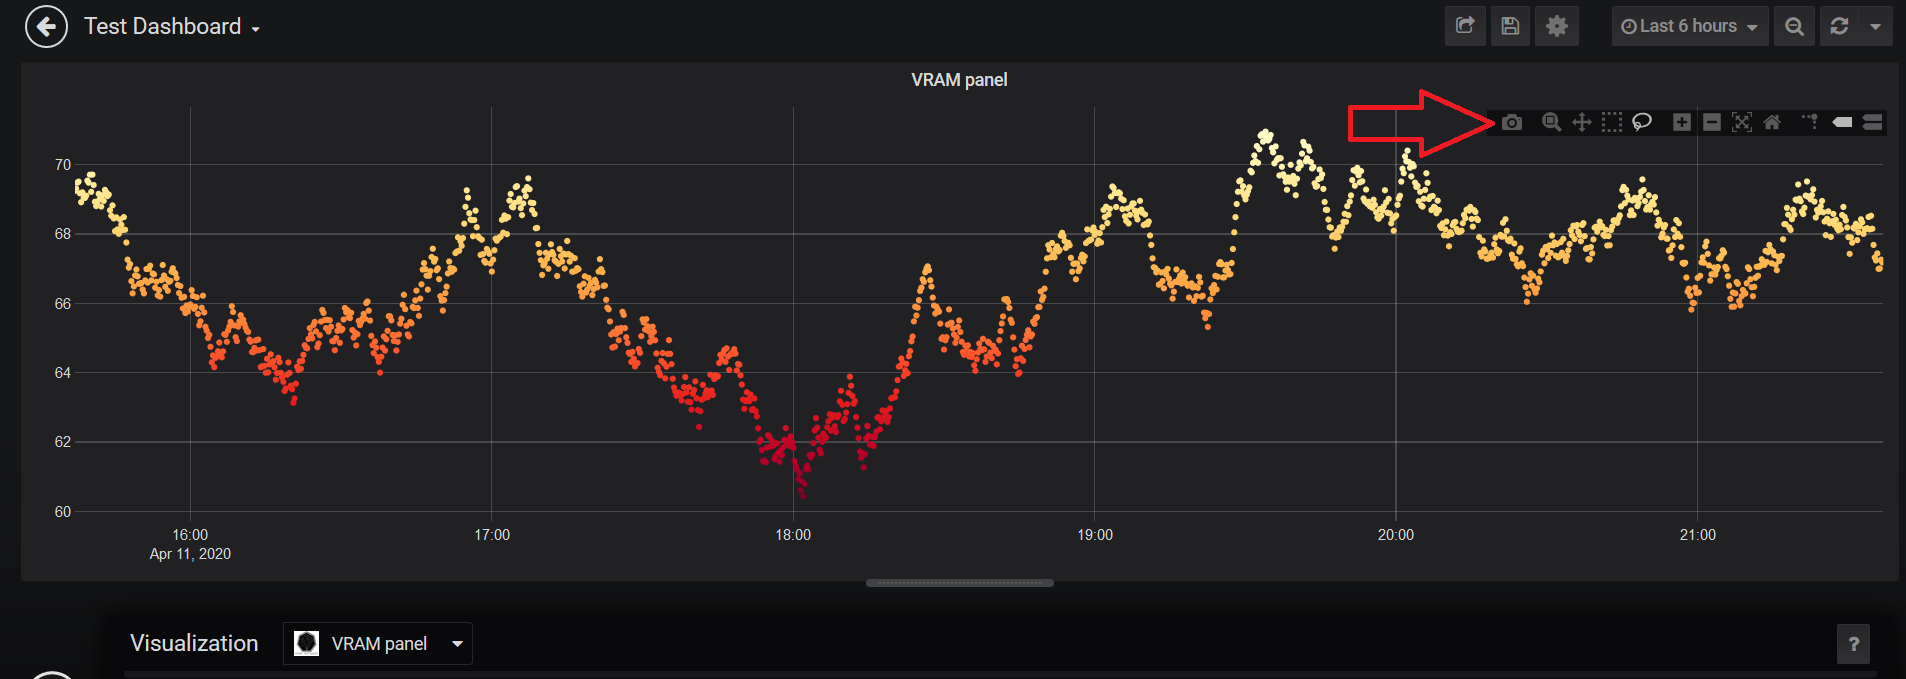
\includegraphics[width=\textwidth,height=\textheight,keepaspectratio]{img/toolbar.png}
            \caption{Toolbar inserita nel grafico}
        \end{figure}
  \pagebreak
	\section{Utilizzo}
	\subsection{Applicazione esterna a Grafana}
		\mbox{}
		\begin{figure} [H]
			\begin{center}
				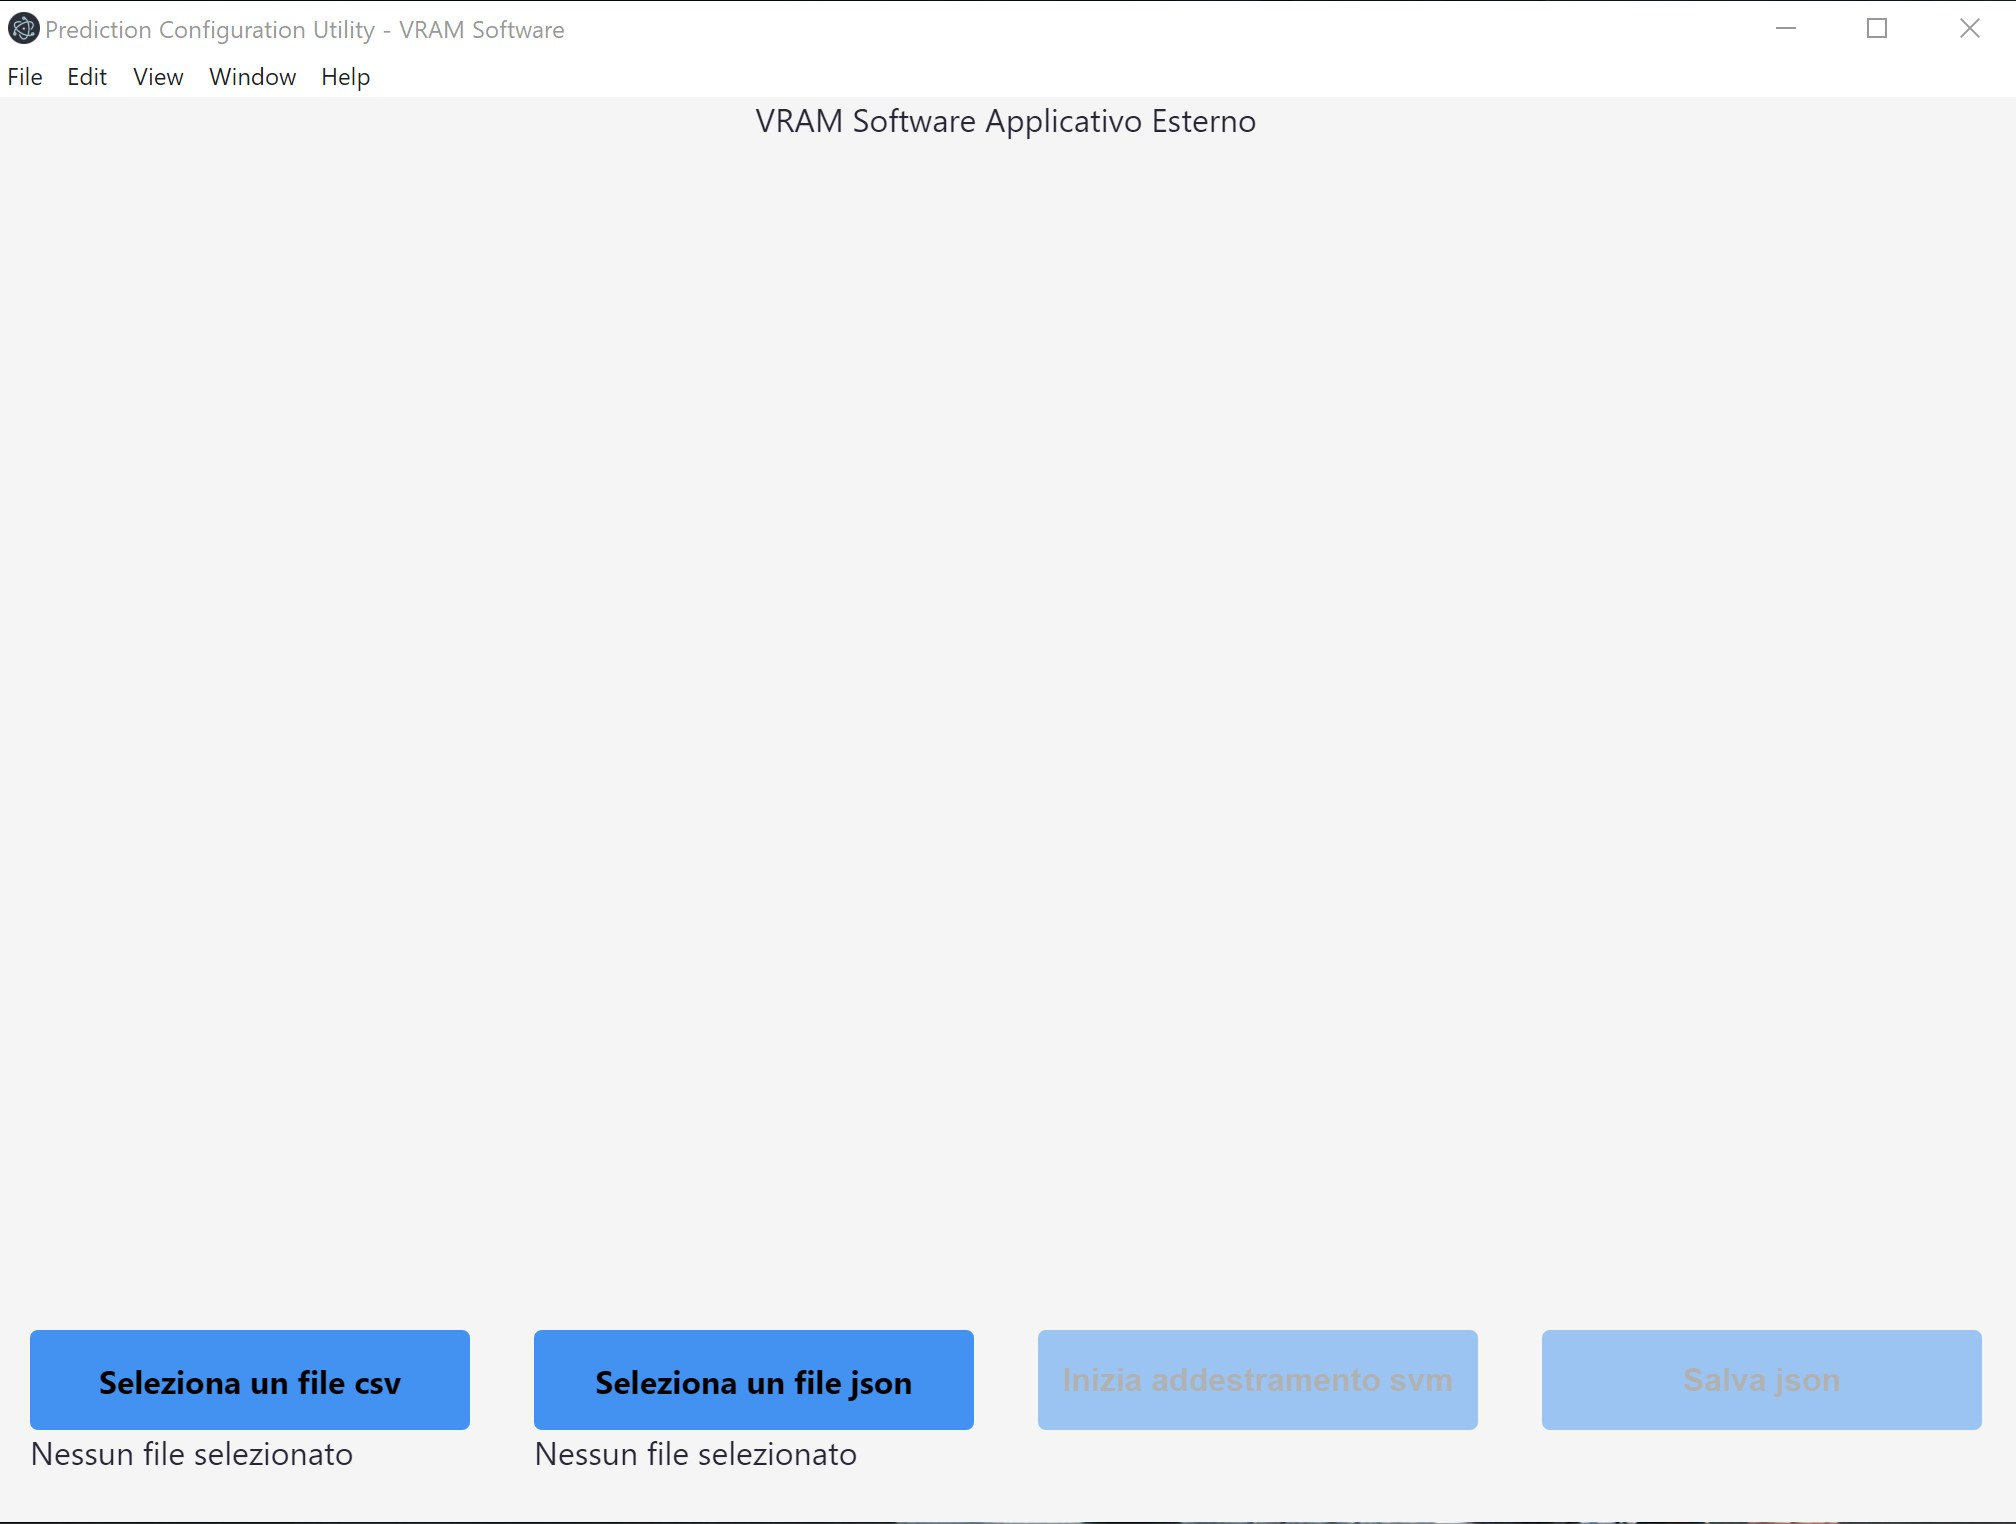
\includegraphics[width=\linewidth]{./img/1.jpg}
			\end{center}
			\caption{Schermata iniziale dell'applicazione esterna}
		\end{figure}
		\mbox{}
		\subsubsection{Aggiunta dei dati di addestramento}
		Per aggiungere i dati di addestramento, cliccare sul pulsante "Seleziona un file csv".
		Si aprirà il file manager di sistema e sarà possibile importare il file desiderato. Una volta selezionato apparirà un pop-up dove sarà possibile scegliere l'algoritmo di predizione che ci desidera addestrare per quei dati, selezionare l'ordine dei predittori e selezionare l'ordine dei predetti.
		\mbox{}
		\begin{figure} [H]
			\begin{center}
				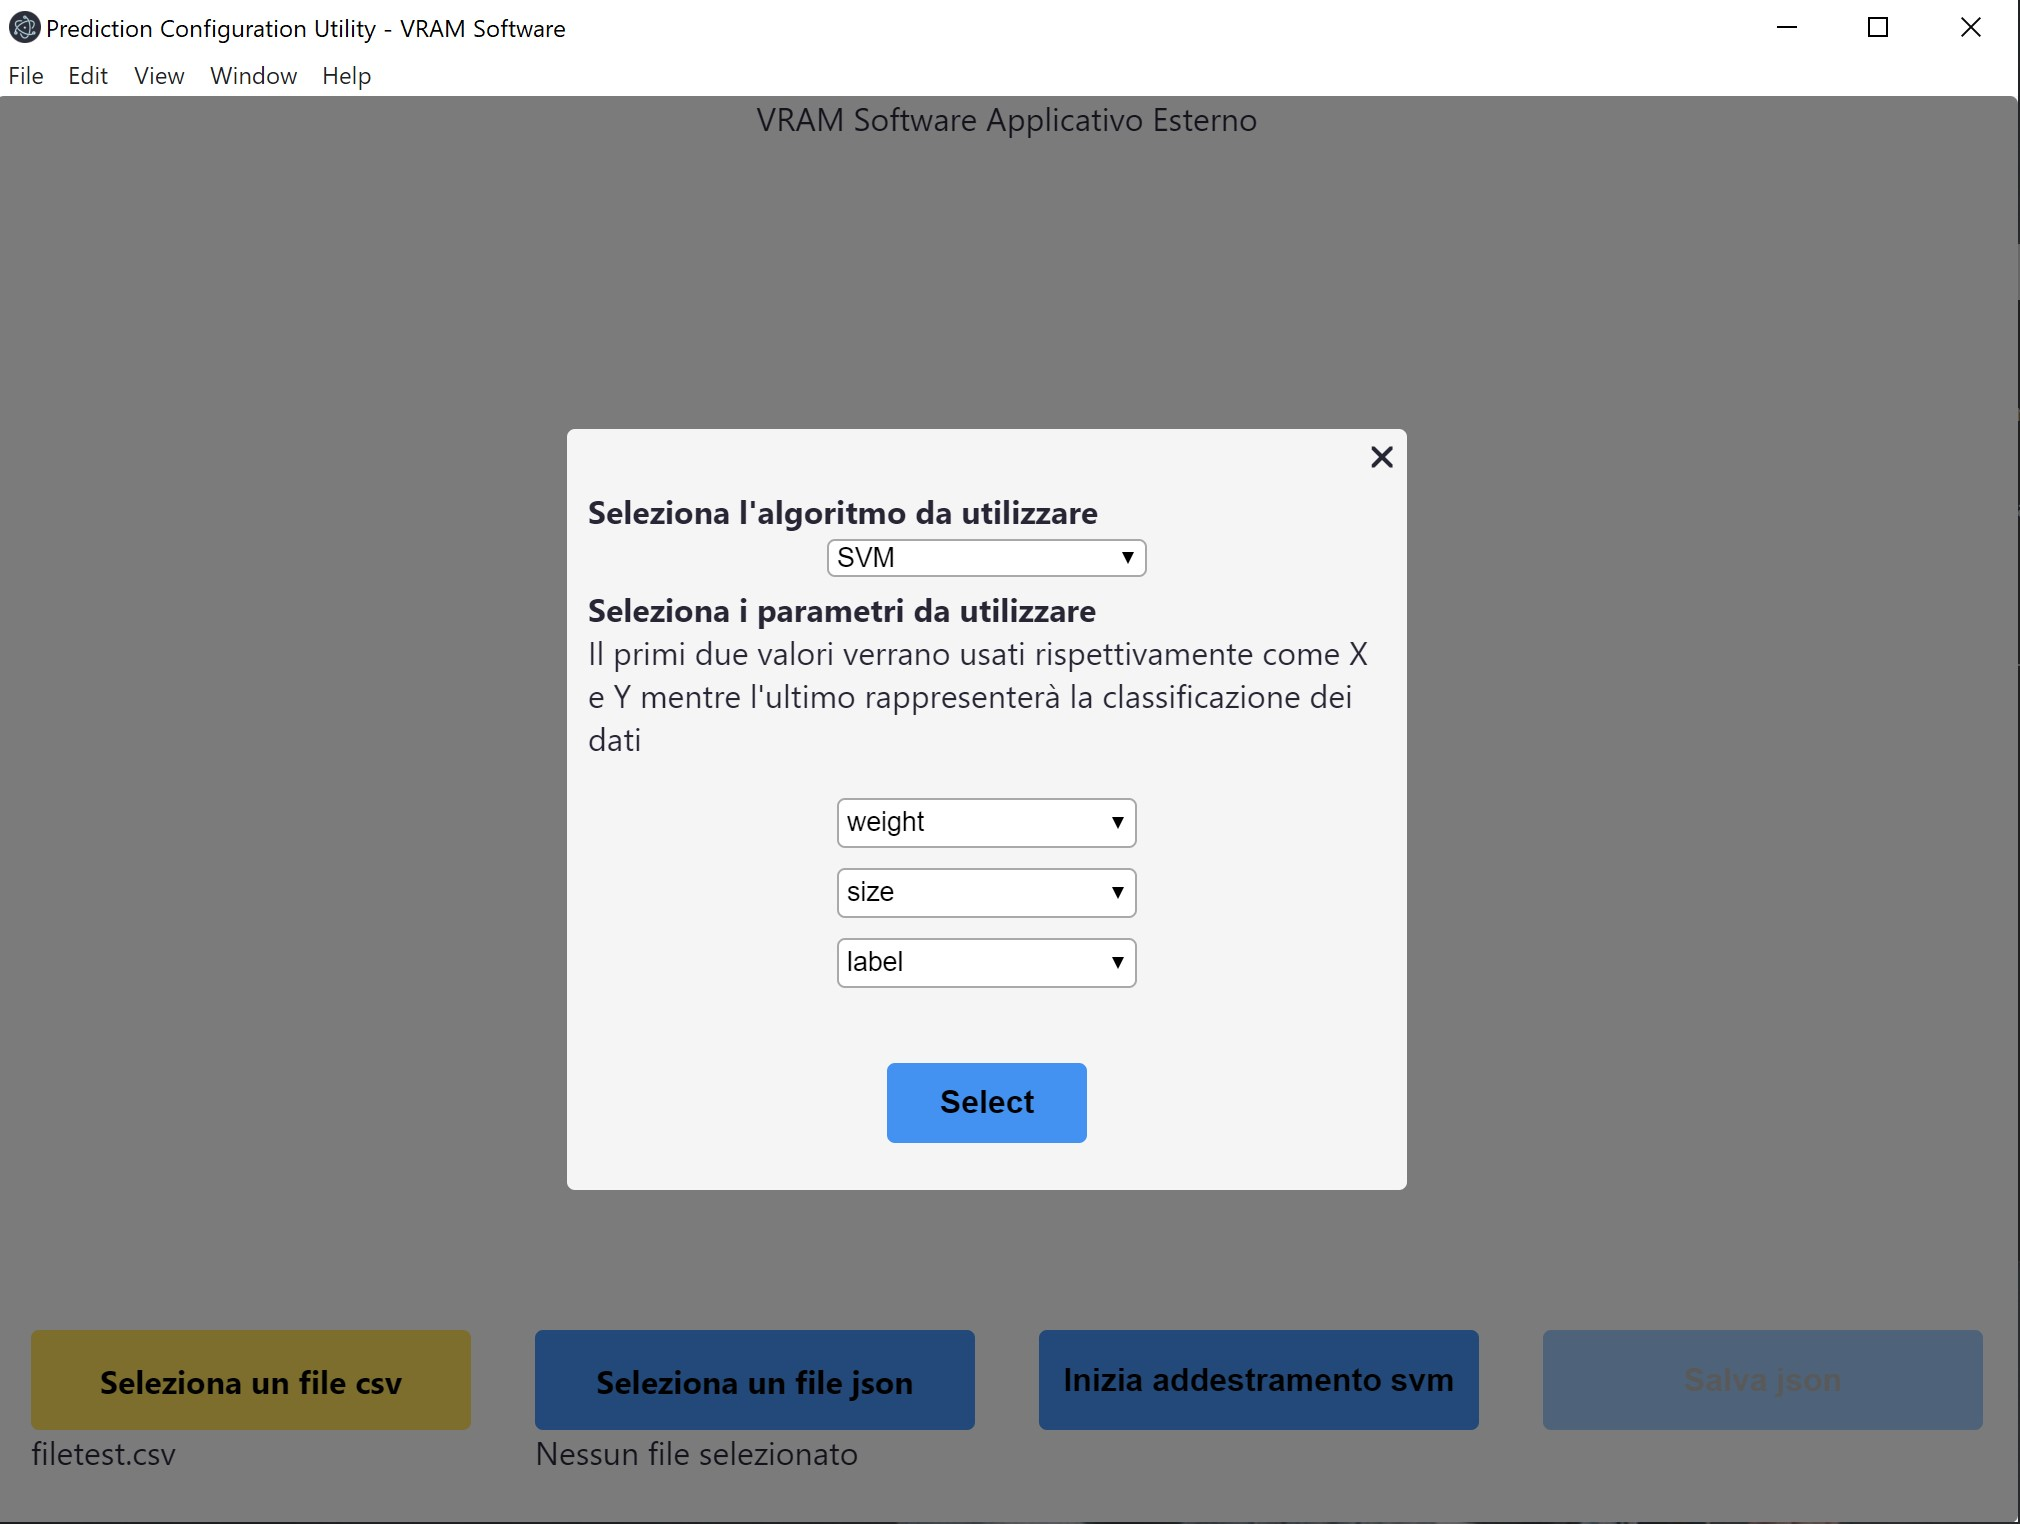
\includegraphics[width=\linewidth]{./img/2.jpg}
			\end{center}
			\caption{Scelta dei parametri}
		\end{figure}
		\mbox{}
		Una volta selezionati apparirà un grafico in base all'ordine scelto.
		\subsubsection{Aggiunta di un file di configurazione}
		Per aggiungere un file di configurazione precedentemente già creato, cliccare sul pulsante "Seleziona un file json".
		Si aprirà il file manager di sistema e sarà possibile importare il file desiderato. Una volta selezionato verranno automaticamente aggiornate le note dell'addestramento.
		\subsubsection{Avvio dell'addestramento}
		Una volta aggiunti i dati di addestramento sarà possibile cliccare sul pulsante "Avvio addestramento". Al termine dell'addestramento verrà visualizzato il messaggio "Addestramento avvenuto" e, se le dimensioni dei dati lo consentono, il risultato sarà visualizzabile nel grafico.
		\mbox{}
		\begin{figure} [H]
			\begin{center}
				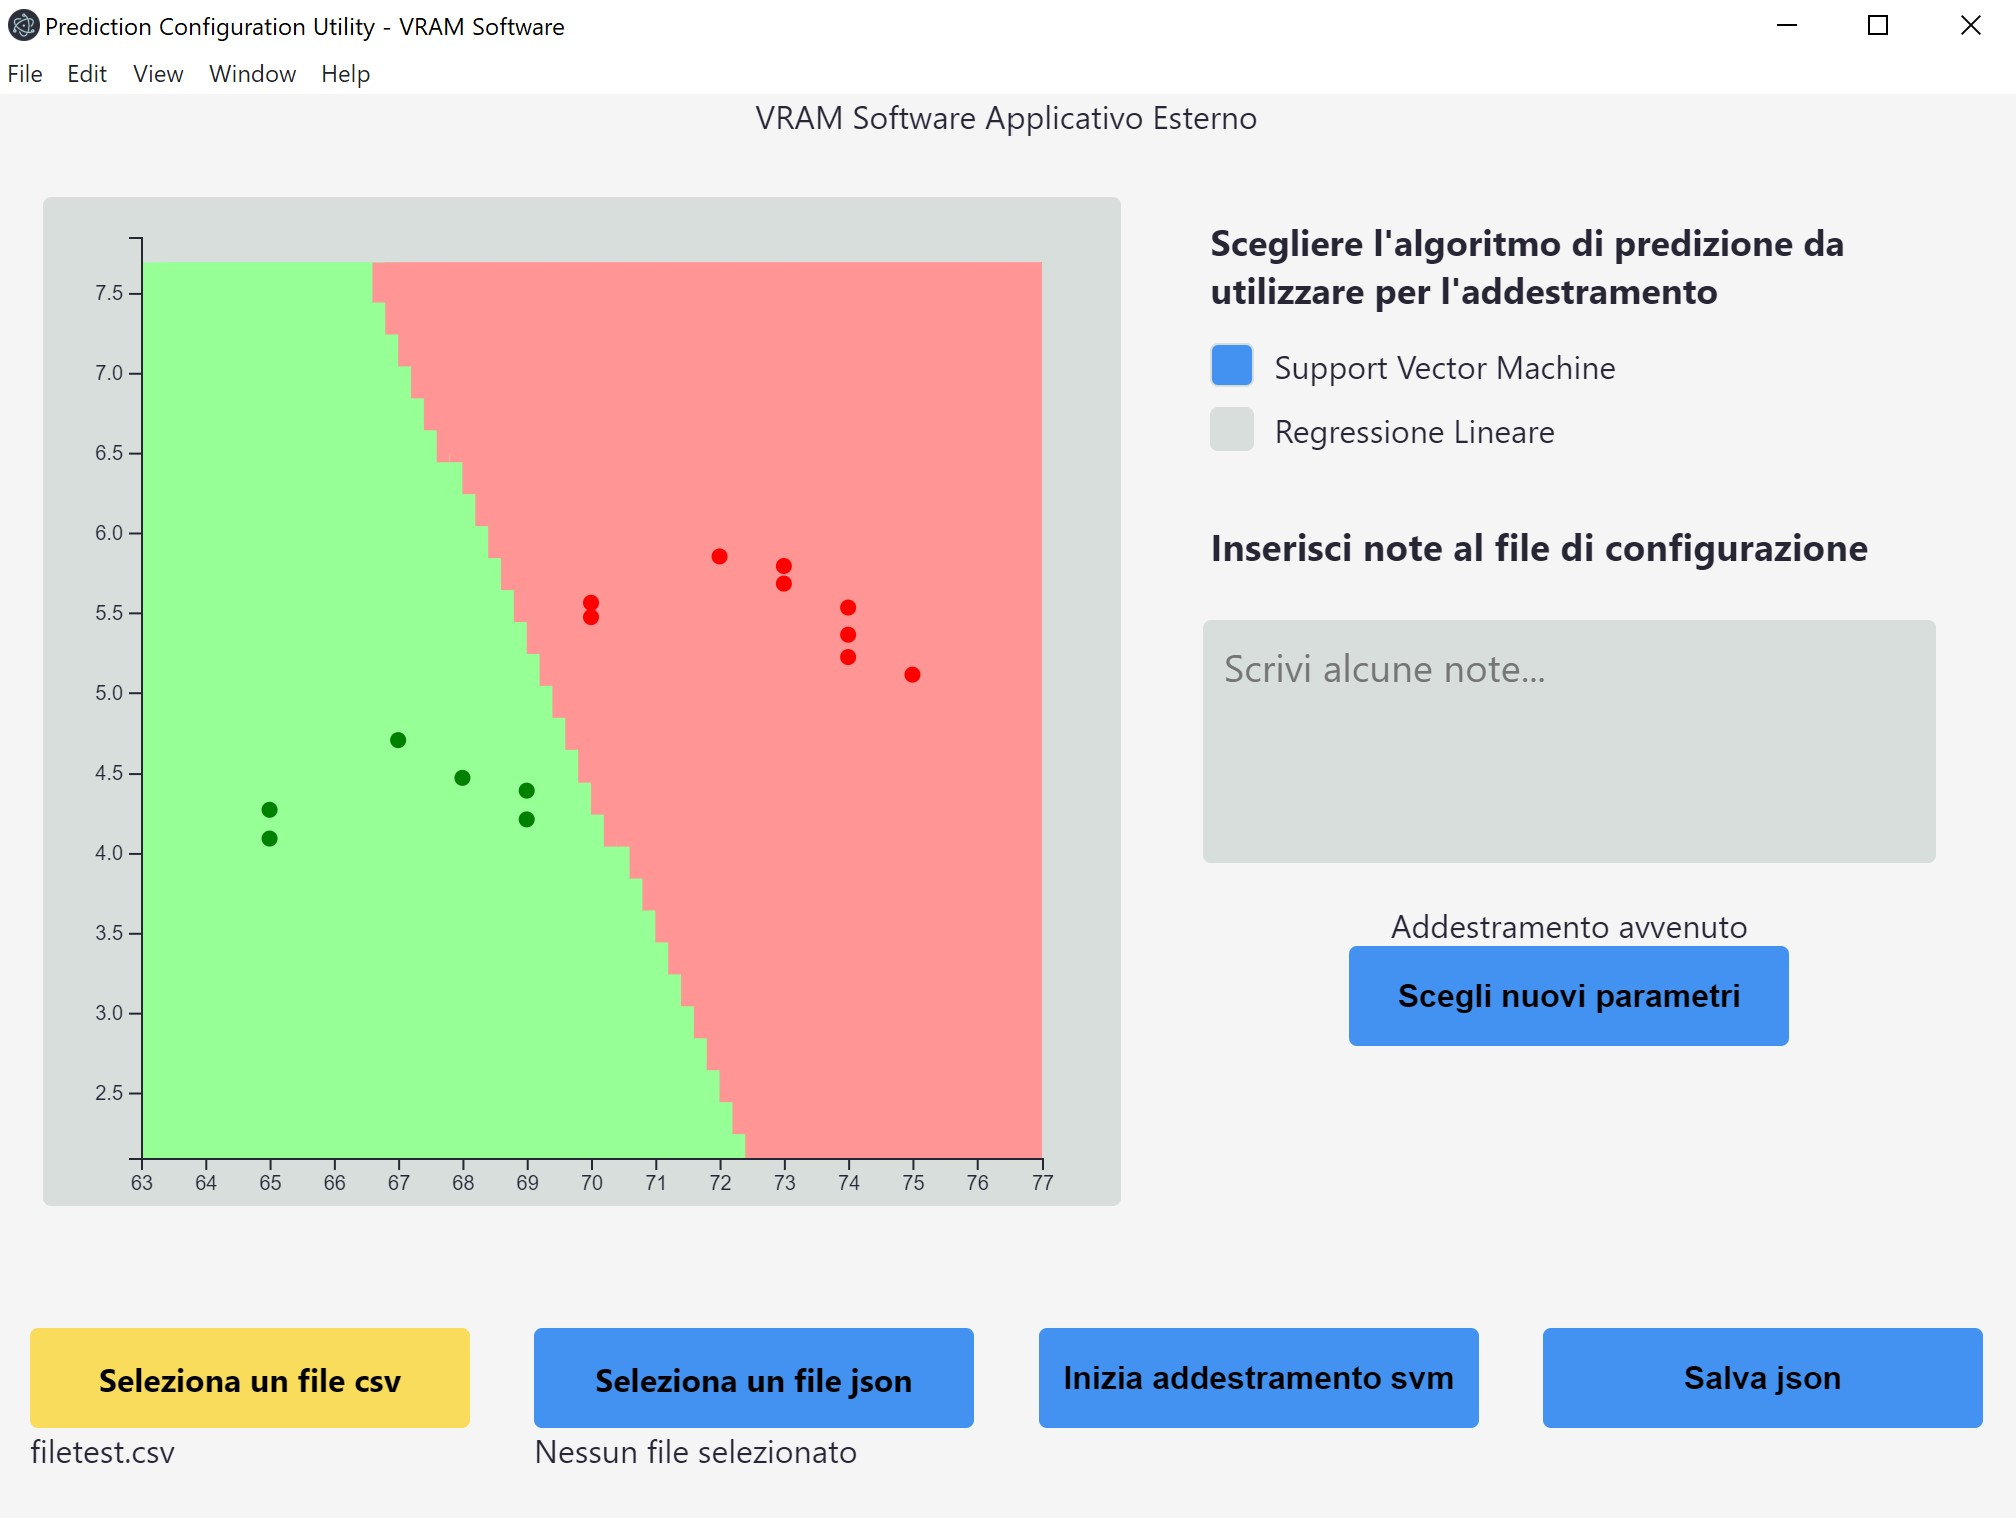
\includegraphics[width=\linewidth]{./img/4.jpg}
			\end{center}
			\caption{Addestramento avvenuto}
		\end{figure}
		\mbox{}
		\subsubsection{Cambio dei parametri}
		Cliccando sul pulsante "Cambia parametri" apparirà un pop-up dove sarà possibile cambiare l'ordine dei predittori e dei predetti come avviene nell'inserimento del file.
		\mbox{}
		\begin{figure} [H]
			\begin{center}
				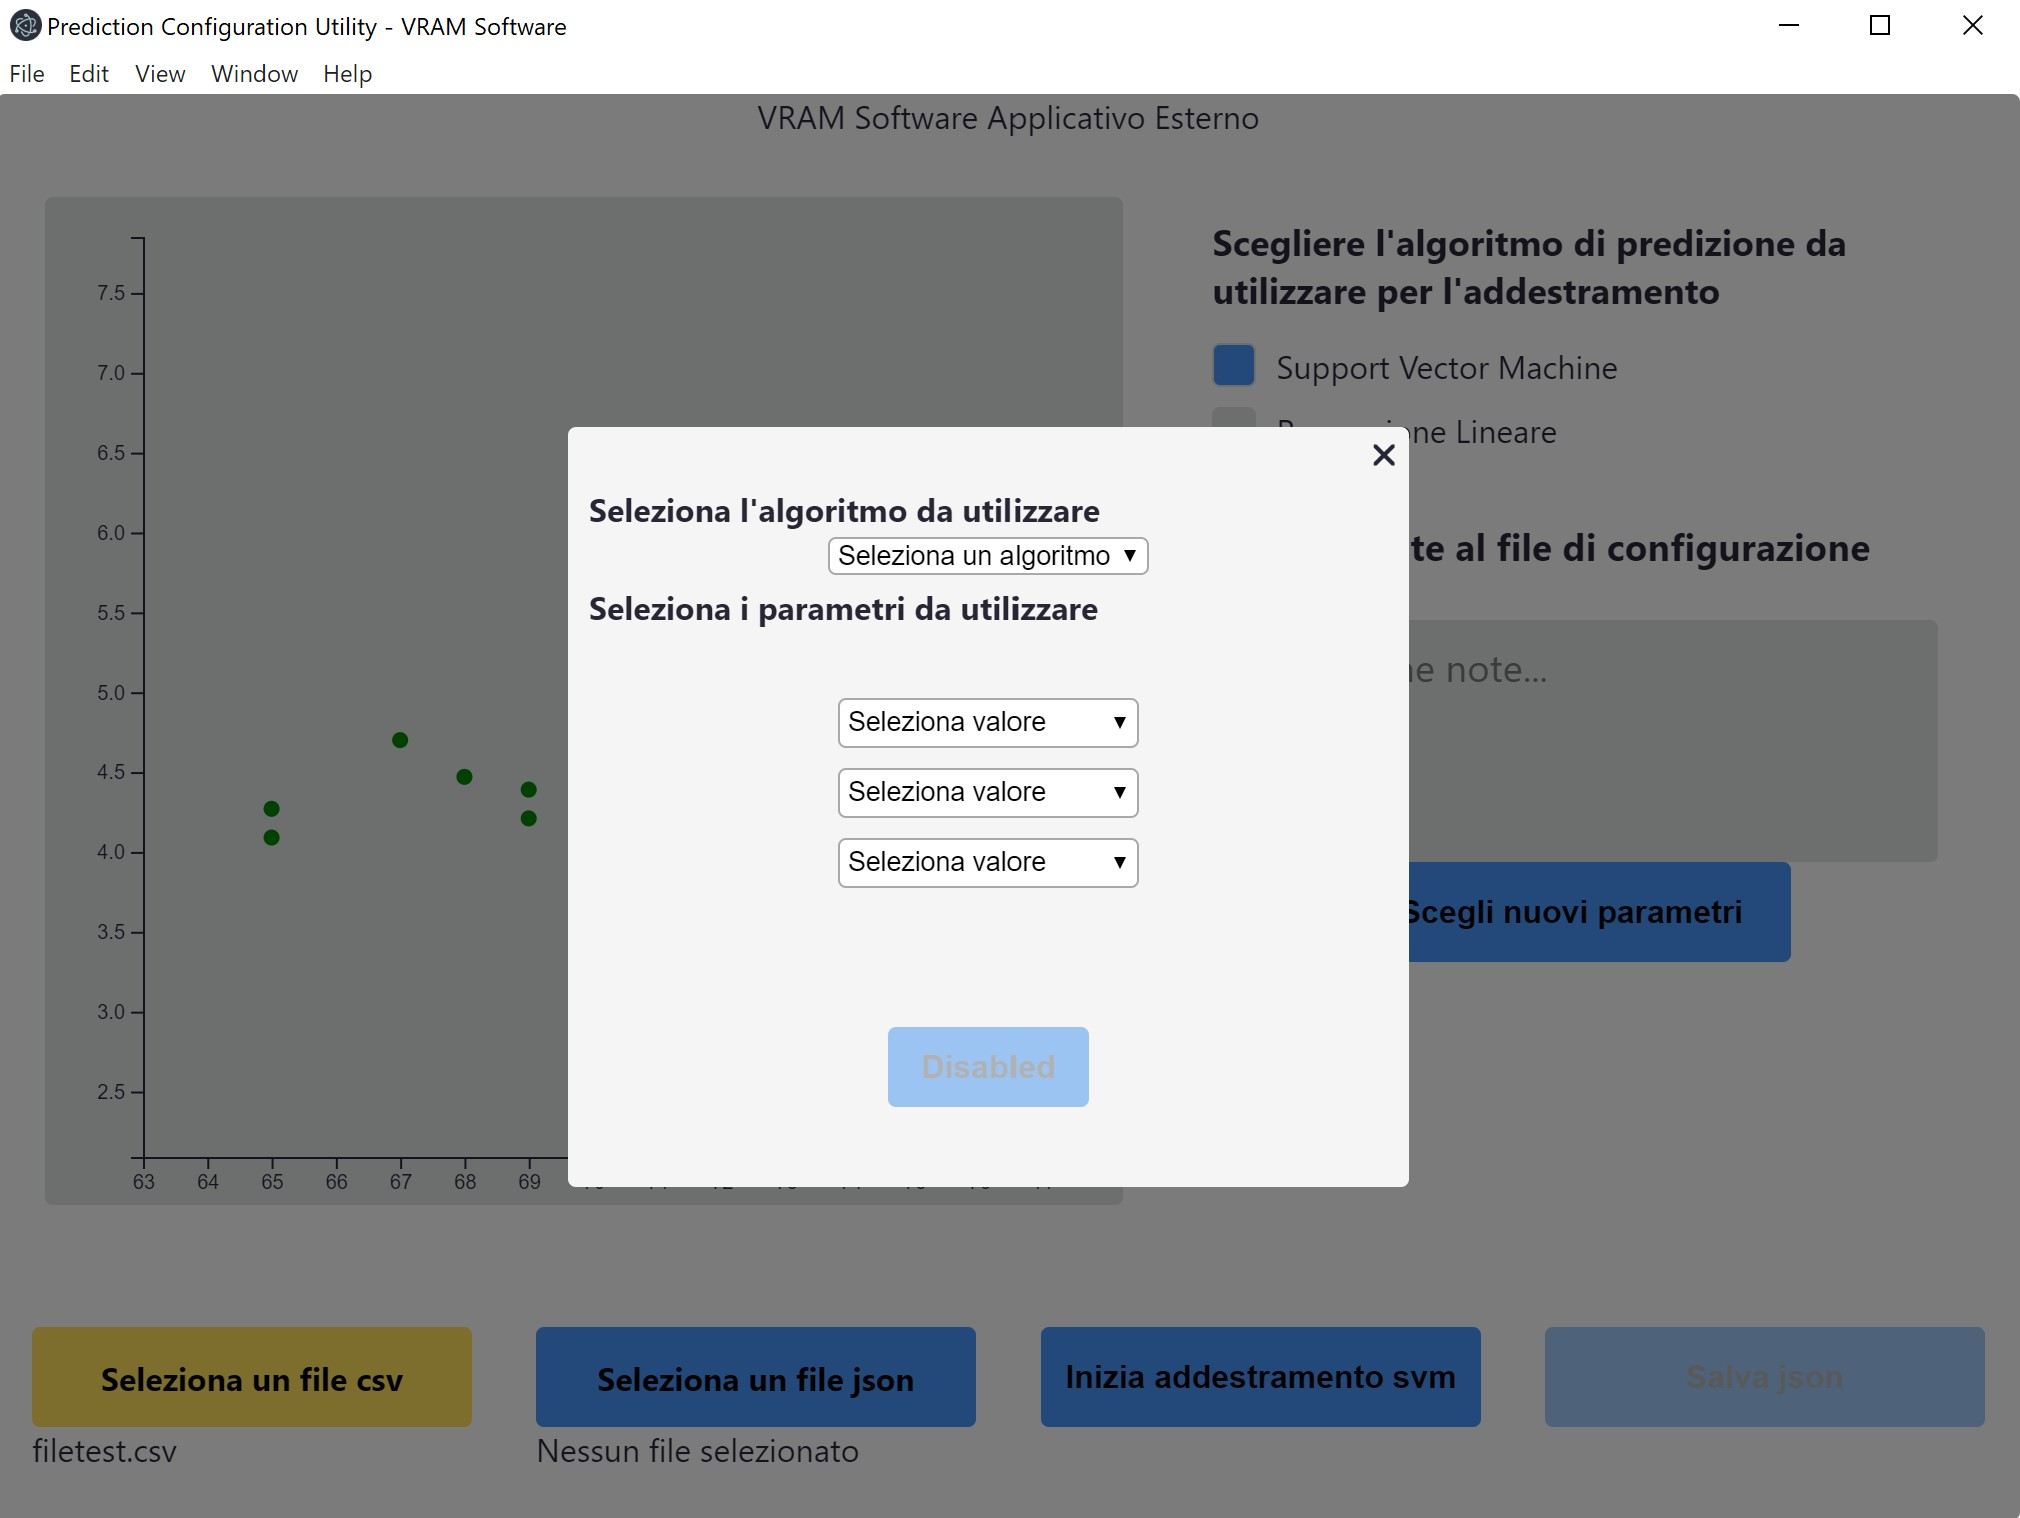
\includegraphics[width=\linewidth]{./img/3.jpg}
			\end{center}
			\caption{Cambio dei parametri}
		\end{figure}
		\mbox{}
		\subsubsection{Salvataggio dei risultati}
		Cliccando sul pulsante "Salva json" apparirà un pop-up in cui si potrà inserire il nome del file e salvarlo sulla cartella "output". Questo file conterrà tutte le informazioni dell'addestramento necessarie per eseguire la predizione e le eventuali note scritte nel box dell'applicazione.
		\mbox{}
		\begin{figure} [H]
			\begin{center}
				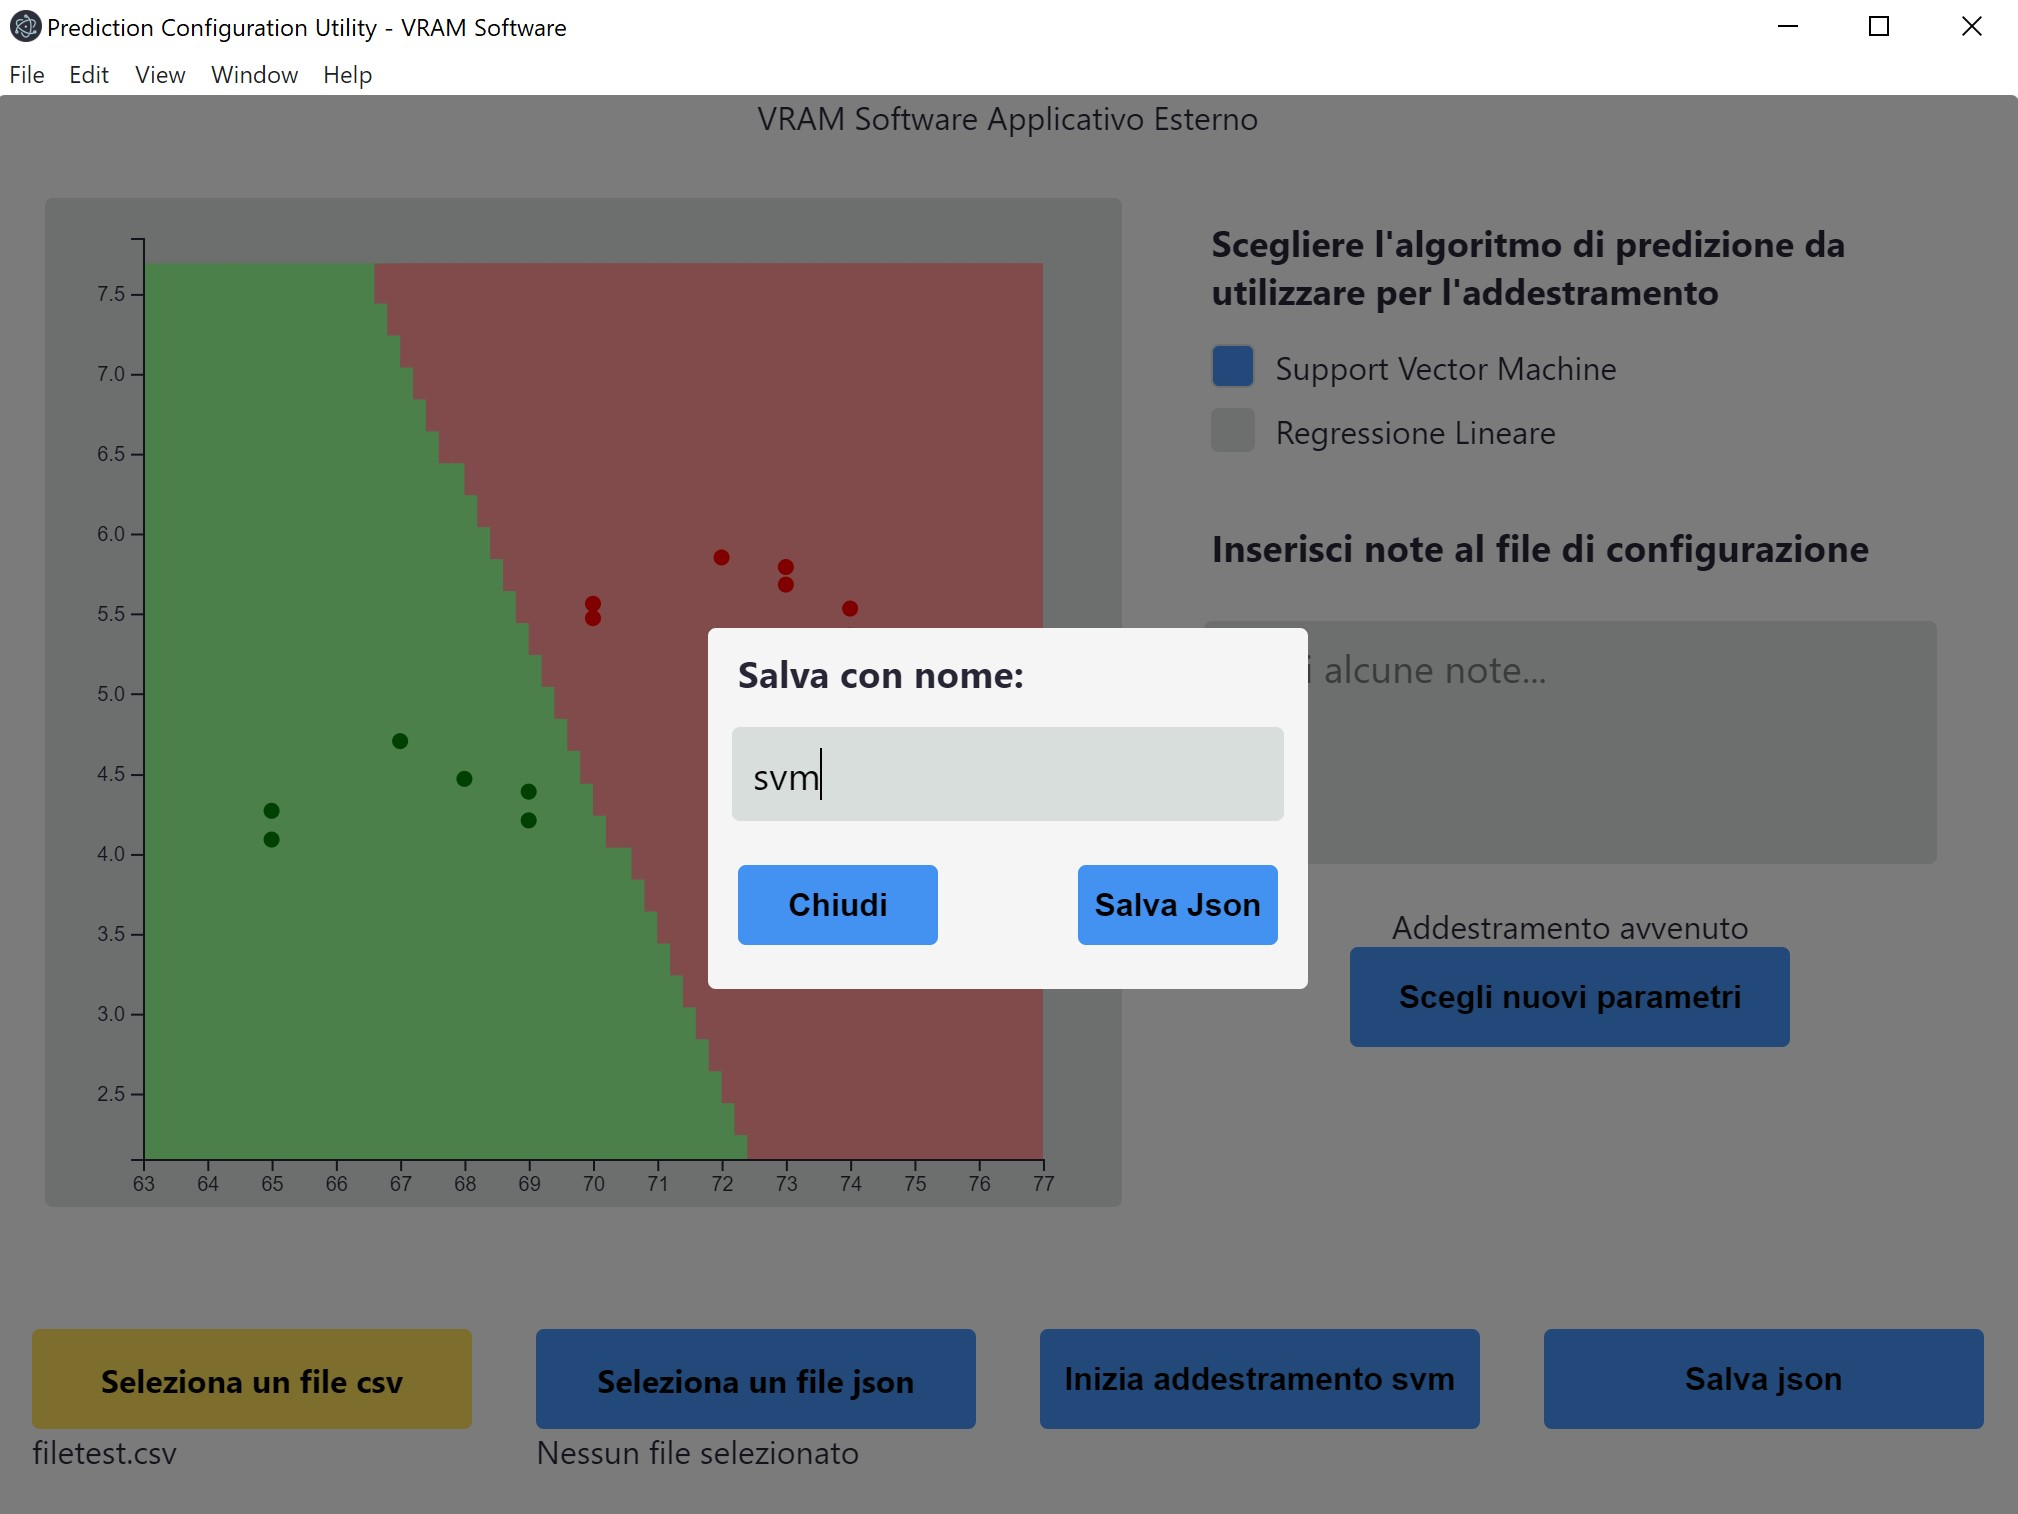
\includegraphics[width=\linewidth]{./img/5.jpg}
			\end{center}
			\caption{Salvataggio del file json contenente la configurazione per la predizione}
		\end{figure}
		\mbox{}
		

	\pagebreak
	\section{Struttura dei file}
	\subsection{Struttura del Json}
	I file Json che contengono la configurazione degli algoritmi di addestramento devono essere strutturati nei modi qui sotto indicati.
		\subsubsection{Regressione Lineare}
		\begin{itemize}
			\item \textbf{author} indica l'autore del file
			\item \textbf{version} indica la versione dell'applicazione con cui si è creato il file
			\item \textbf{date} indica la data in cui è stato creato il file
			\item \textbf{time} indica l'ora in cui è stato creato il file
			\item \textbf{pluginAim} indica l'algoritmo addestrato, in questo caso deve essere "rl"
			\item \textbf{predictors} elenco delle etichette dei predittori
			\item \textbf{result} elenco dei coefficienti risultati dall'addestramento
			\item \textbf{notes} eventuali note inserite durante l'addestramento
		\end{itemize}
		\mbox{}
		\begin{figure} [H]
			\begin{center}
				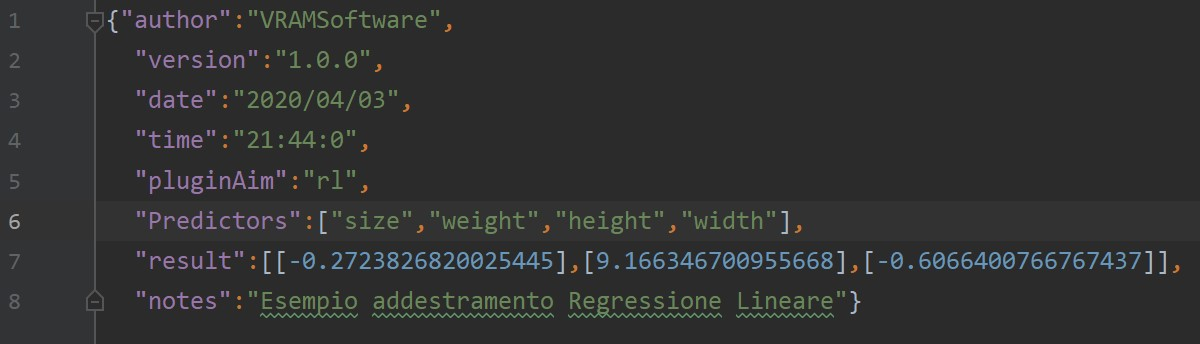
\includegraphics[width=\linewidth]{./img/jsonRl.jpg}
			\end{center}
			\caption{Esempio file Json per la Regressione Lineare}
		\end{figure}
		\mbox{}
		\subsubsection{Support Vector Machine}
			\begin{itemize}
				\item \textbf{author} indica l'autore del file
				\item \textbf{version} indica la versione dell'applicazione con cui si è creato il file
				\item \textbf{date} indica la data in cui è stato creato il file
				\item \textbf{time} indica l'ora in cui è stato creato il file
				\item \textbf{pluginAim} indica l'algoritmo addestrato, in questo caso deve essere "svm"
				\item \textbf{predictors} elenco delle etichette dei predittori
				\item \textbf{trainData} elenco dei dati addestrati
				\item \textbf{trainLabels} elenco delle label dei dati addestrati
				\item \textbf{result} elenco dei parametri risultati dall'addestramento, in particolare 
				\begin{itemize}
					\item \textbf{N} indica il numero di dati addestrati
					\item \textbf{D} indica la dimensione dei dati addestrati
					\item \textbf{b} indica lo scalare risultato dall'addestramento
					\item \textbf{kernelType} indica il tipo di kernel utilizzato, attualmente è implementato solo il kernel "linear"
					\item \textbf{w} indica il vettore risultato dall'addestramento					
				\end{itemize}
				\item \textbf{notes} eventuali note inserite durante l'addestramento
			\end{itemize}
		\mbox{}
		\begin{figure} [H]
			\begin{center}
				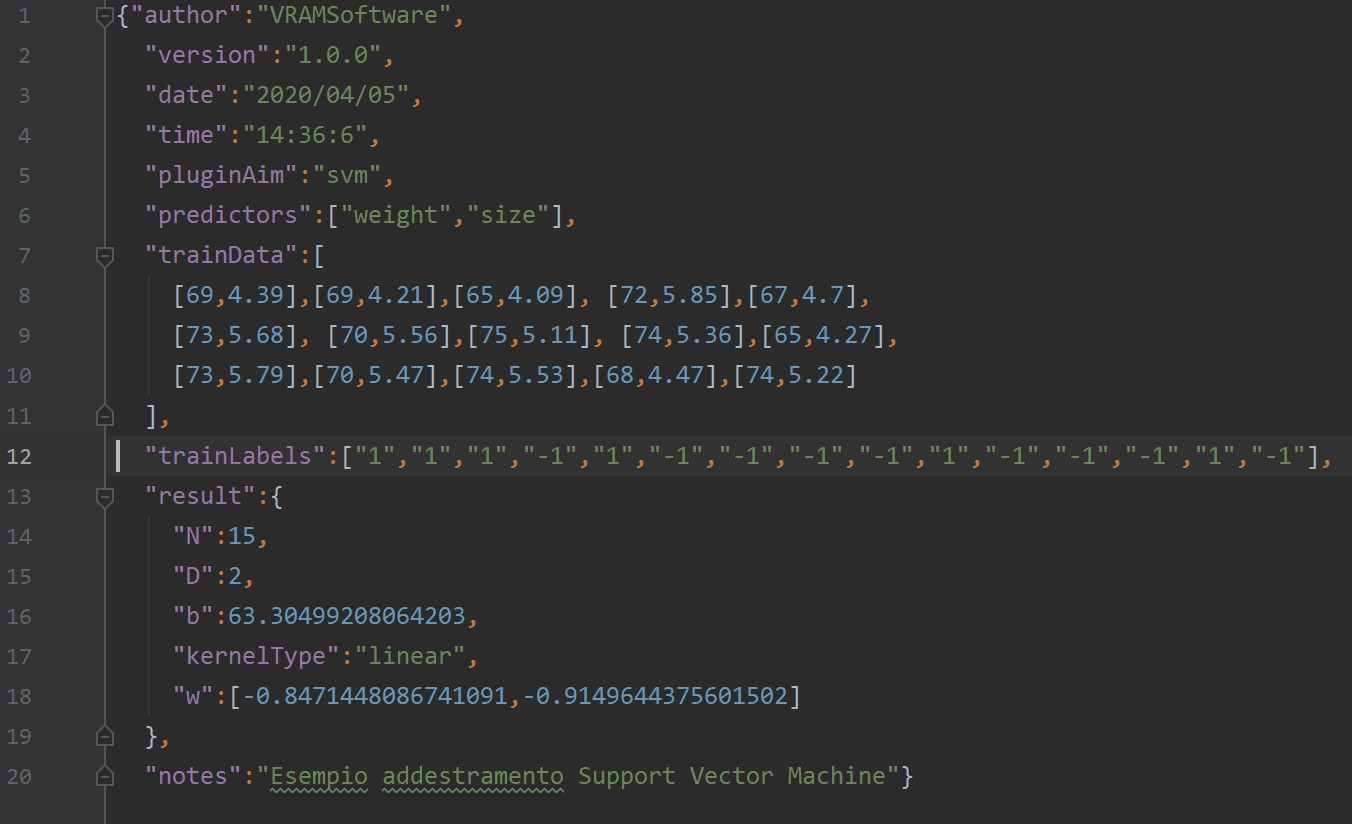
\includegraphics[width=\linewidth]{./img/jsonSvm.jpg}
			\end{center}
			\caption{Esempio file Json per la Support Vector Machine}
		\end{figure}
		\mbox{} \\ \\ 
		Se si desiderano ulteriori informazioni sulle regole sintattiche dei file JSON, si consiglia di consultare la documentazione W3C disponibile al seguente link:
		\\[0.2cm]
		\hspace*{10mm}
		\url{https://www.w3schools.com/js/js_json_syntax.asp}
		
	\subsection{Struttura del CSV}
	La struttura del file .csv è indipendente dall'algoritmo che si vuole addestrare.
	Deve presentare i valori di ogni predittore divisi per colonne, la prima riga di ogni colonna deve indicare l'etichetta associata al predittore. \\
	A seconda del caso devono essere presenti una o più colonne per i predetti, la prima riga di ogni colonna deve indicare l'etichetta associata al predetto.
	\mbox{}
	\begin{figure} [H]
		\begin{center}
			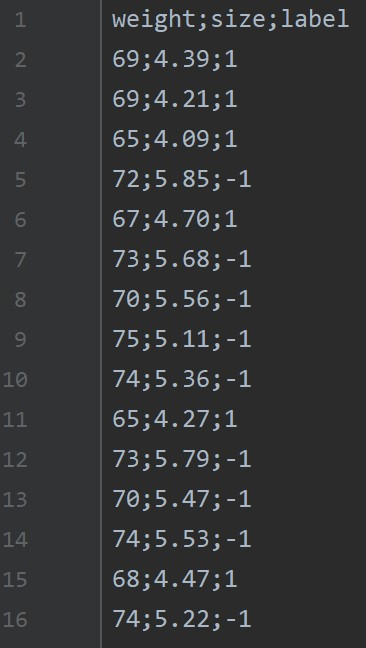
\includegraphics[width=50mm]{./img/csv1.jpg}
		\end{center}
		\caption{Esempio file csv}
	\end{figure}
	\mbox{}
	I file .csv possono eventualmente essere gestiti tramite fogli di calcolo
	\mbox{}
	\begin{figure} [H]
		\begin{center}
			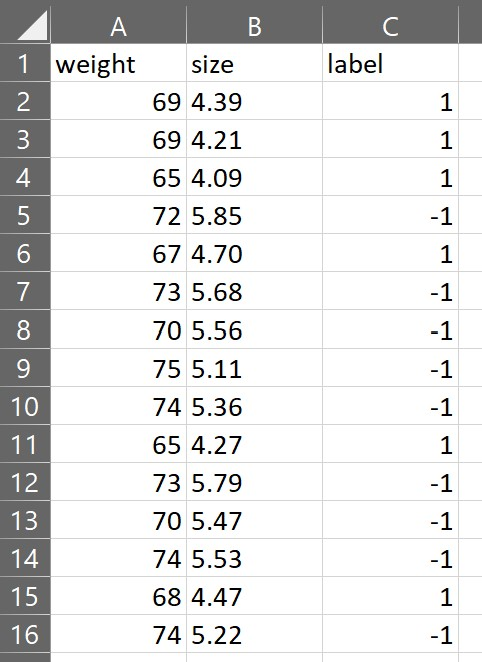
\includegraphics[width=50mm]{./img/csv2.jpg}
		\end{center}
		\caption{Esempio file csv su Microsoft Excel}
	\end{figure}
	\mbox{} 
	\pagebreak
	\section{Segnalazione errori}
Nel caso si riscontrassero anomalie o errori durante l'esecuzione del plug-in o dell'applicazione di addestramento, è possibile segnalarli tramite l'indirizzo email {\url{vram.software@gmail.com}}.
	\subsection{Segnalazione errori nell'applicazione di addestramento}
	Indicare nell'oggetto [BUG][AppAddestramento] se si vuole segnalare la presenza di un bug nell'applicazione di addestramento.
	Nel corpo della mail indicare:
	\begin{itemize}
		\item versione dell'applicazione di addestramento;
		\item sistema operativo e relativa versione;
		\item descrizione dettagliata dell'errore riscontrato.
	\end{itemize}
	\mbox{}
	\begin{figure} [H]
		\begin{center}
			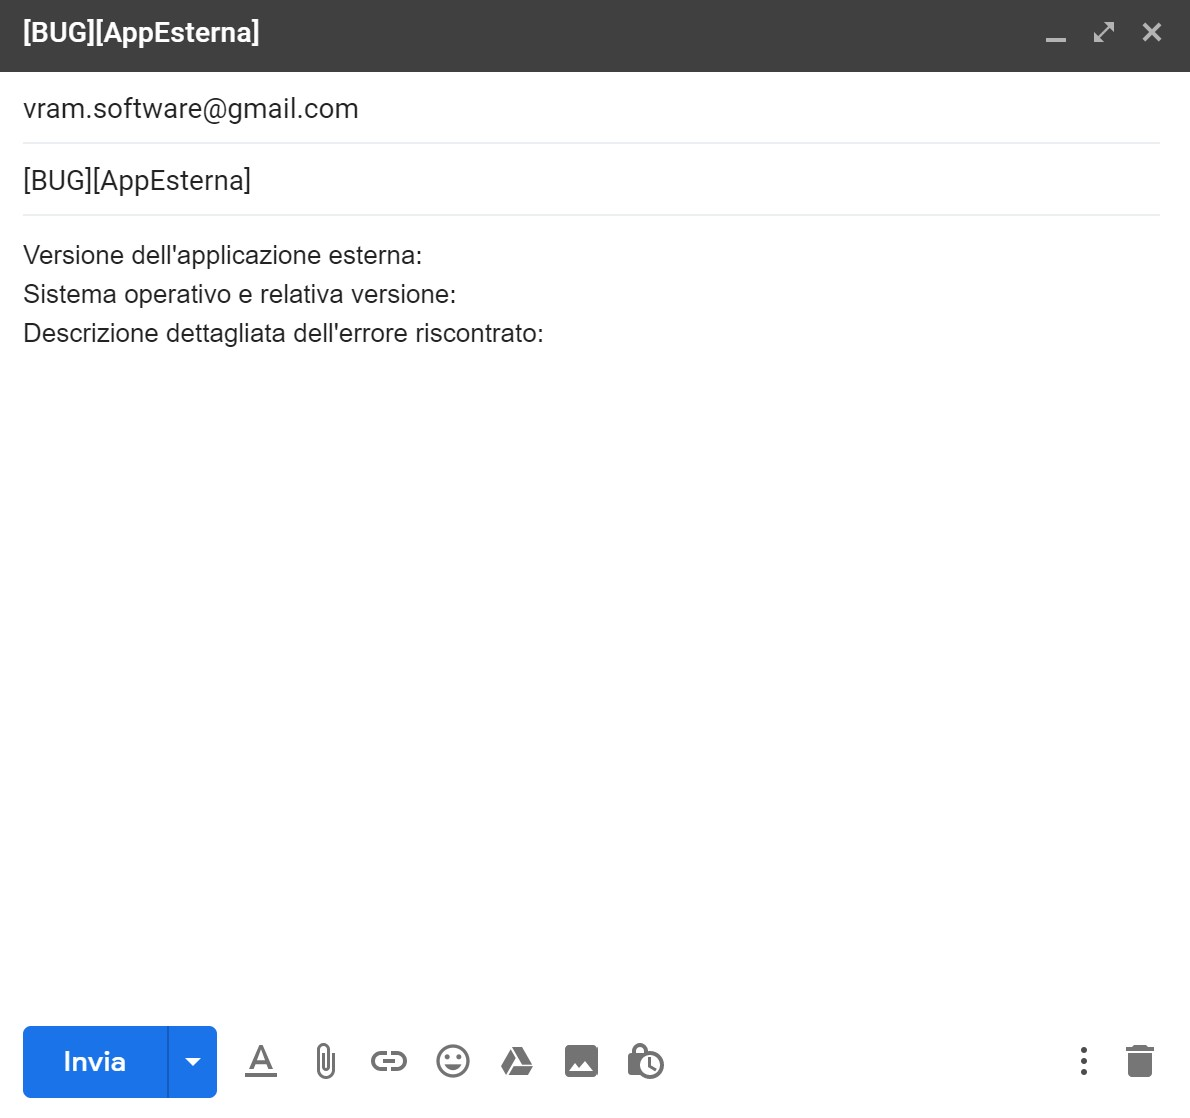
\includegraphics[width=120mm]{./img/erroriApp.jpg}
		\end{center}
		\caption{Template email segnalazione errori nell'applicazione di addestramento}
	\end{figure}
	\mbox{}
	\subsection{Segnalazione errori nel plug-in}
 	[BUG][Plug-in] se si vuole segnalare la presenza di un bug nel plug-in.
 	Nel corpo della mail indicare:
 	\begin{itemize}
 		\item versione del plug-in;
 		\item versione di Grafana\glo;
 		\item sistema operativo e relativa versione;
 		\item browser utilizzato e relativa versione;
 		\item descrizione dettagliata dell'errore riscontrato.
 	\end{itemize}
 	\mbox{}
 	\begin{figure} [H]
 		\begin{center}
 			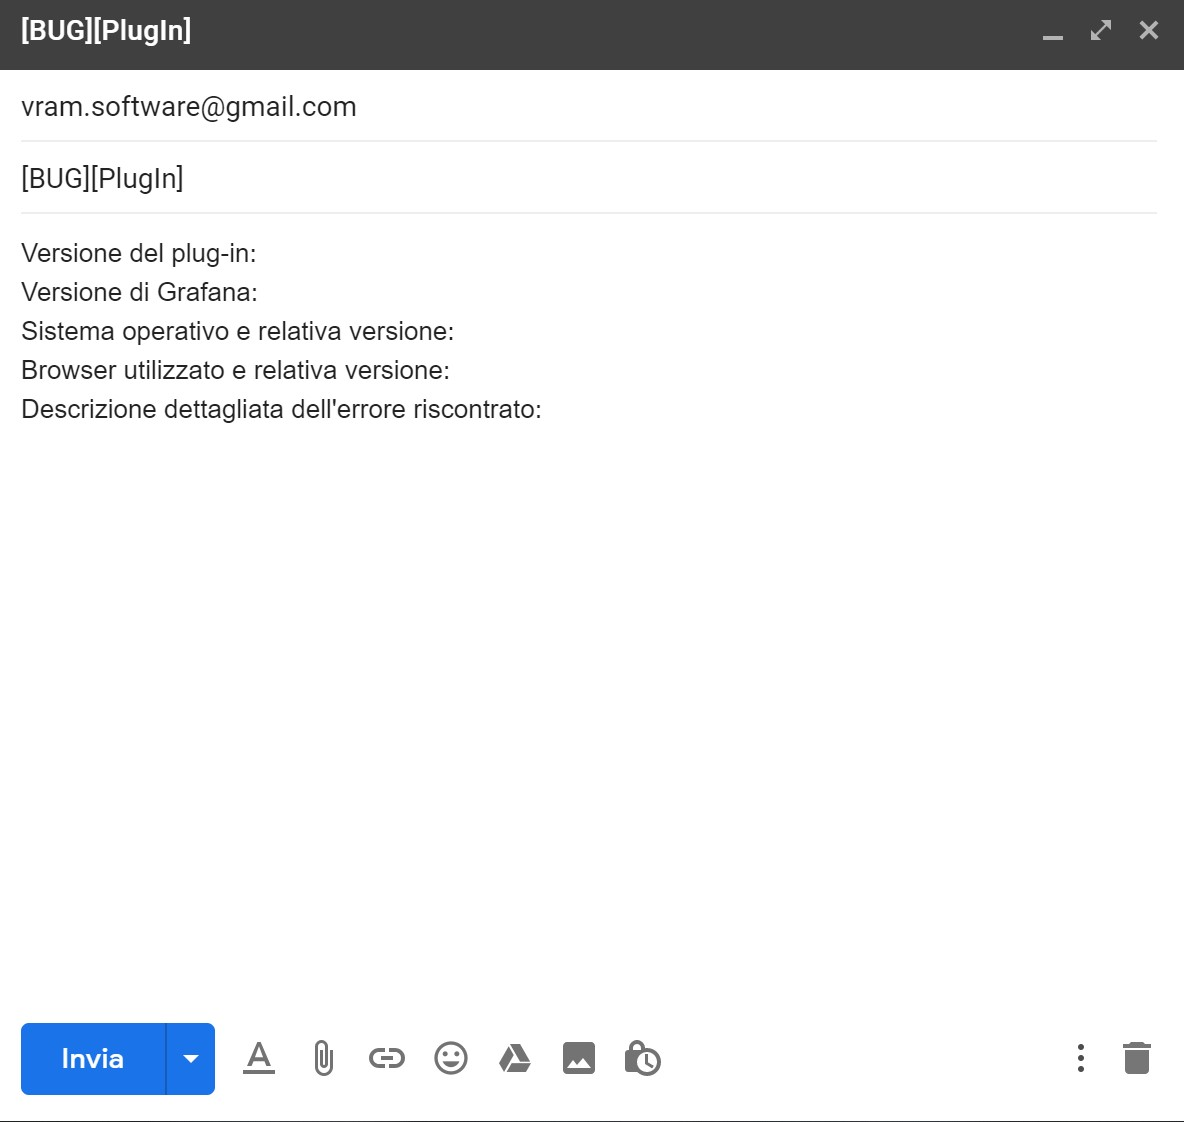
\includegraphics[width=120mm]{./img/erroriPlugIn.jpg}
 		\end{center}
 		\caption{Template email segnalazione errori nel plug-in}
 	\end{figure}

	
	\appendix
	\pagebreak
	\section{Glossario}

%\subsection*{C}
%\subsubsection*{CSV}
%Il comma-separated values (abbreviato in CSV) è un formato di file basato su file di testo utilizzato per l'importazione ed esportazione di una tabella di dati. 

\subsection*{D}
\subsubsection*{Datasource}
Una datasource è una sorgente di dati in Grafana. Solitamente si tratta di un database.

\subsubsection*{Dashboard}
In italiano cruscotto; interfaccia che permette all'utente di tenere sotto controllo gli indicatori più importanti dell'ambiente in cui sta lavorando. È caratteristica fondamentale l'aggiornamento automatico dei dati, senza che vi debba essere un'interazione con l'utente.

\subsection*{G}
\subsubsection*{Grafana}
Software ad uso generico per la produzione di cruscotti informativi (dashboard in inglese) e composizione di grafici. Viene utilizzato come un'applicazione web.

\subsection*{I}
\subsubsection*{InfluxDB}
InfluxDB è un database basato sul concetto di serie temporale. InfluxDB è specializzato e
ottimizzato per il salvataggio e la lettura di serie temporali: record salvati in ordine temporale
e caratterizzati dal timestamp, ovvero un campo che indica una data. InfluxDB è utilizzato
per lo più in ambiti in cui è necessario salvare valori generati da sensori oppure analytics in
tempo reale.

%\subsection*{J}
%\subsubsection*{JSON}
%Acronimo di JavaScript Object Notation, è un formato adatto all'interscambio di dati fra applicazioni client/server. È basato sul linguaggio JavaScript Standard ma ne è indipendente.

\subsection*{M}
\subsubsection*{Machine learning}
Il machine learning (in italiano apprendimento automatico) è una branca dell'intelligenza artificiale che utilizza metodi statistici per migliorare progressivamente la performance di un algoritmo nell'identificare pattern nei dati.

\subsection*{P}
\subsubsection*{Predittore}
Dati o variabili su cui applico le tecniche di regressione o di classificazione per ottenere un dato la cui diretta rilevazione sarebbe impossibile o troppo onerosa.

\subsubsection*{Prodotto}
Si definisce prodotto qualsiasi bene scambiabile sul mercato che può rispondere alle esigenze di un compratore. Un esempio di prodotto informatico è il software che è composto dal codice e dalla documentazione.	

\subsubsection*{RL}
Acronimo di Regressione lineare, algoritmo di machine learning\glosp che ha la funzione di prevedere un valore di una variabile dipendente (y) in base a una determinata variabile indipendente (x) secondo una relazione di tipo lineare.
\subsection*{S}
\subsubsection*{SVM}
Acronimo di Support Vector Machine; algoritmo di apprendimento automatico supervisionato che può essere utilizzato sia per scopi di classificazione che di regressione.


	%Tutte le sezioni del documento
	%\input{res/inserire nome sezione 1} 
	% ...
	%\input{res/inserire nome sezione n} 
\end{document}